\documentclass{article}

\usepackage{ctex}
\usepackage{listings}
\usepackage[framed,numbered,autolinebreaks,useliterate]{mcode}
\usepackage{geometry}
\usepackage{multirow}
\usepackage{graphicx}
\usepackage{amsmath}
\usepackage{float}
\geometry{a4paper, scale=0.8}

\title{数学实验实验报告}
\author{ZhaohengLi 2017050025\\cainetatum@foxmail.com\\15801206130}

\begin{document}
\maketitle
\section{实验目的}
\begin{itemize}
	\item{了解回归分析的基本原理,并学会解决实际问题;}
	\item{练习使用 MATLAB 解决实际问题。}
\end{itemize}


\section{CH13-T7 耗氧能力}
\subsection{模型设计与建立}
本题不同小问需要建立不同的模型,由于提供信息较少,难以做出精确符合现实情况的模型,因此这里使用最简单的线性回归法进行拟合,模型基本形式如下:

$$y=\beta_0+\beta_1x_1+\cdots+\beta_mx_m+\sum_{i\leq j,k\leq m}\beta_{jk}x_jx_k+\xi$$

通过计算发现,高次项和交互项对题目意义不大,因此所给定的5个自变量和因变量之间的关系比较模糊,几个变量的彼此关系也很难说清楚,因此用自变量的一次线性拟合就可以满足题目要求。但作为实验练习过程,还是将每种回归方法都是使到了,可以作为参考。

\subsection{算法设计与实现}

代码以及注释如下:

\begin{lstlisting}
%% Data
clear
A = ...
n = 24
y = A(2,:);
x1 = A(3,:); x2 = A(4,:); x3 = A(5,:); x4 = a(6,:); x5 = A(7,:);

%% Plot
for i = 1:5
	subplot(2,3,i),plot(A(i+2,:),y,'+'),grid
	pause
end
pause

%% 单参数回归(第一问)
X=[ones(n,1),x4'];
[b,bint,r,rint,s]=regress(y',X);
b,bint,s,
rcoplot(r,rint)
Polytool(x3',y',2)

%% 双参数回归(第二问)
X=[x1',x2',x3',x4',x5'];
stepwise(X5,y');
XX=[x3',x1'];
rstool(XX,y','linear')

%% 全部参数回归(第三问)
X5=[x1',x2',x3',x4',x5'];
stepwise(X5,y')

\end{lstlisting}

第五问要求对残差进行分析,并且剔除异常点,可以在该问的到最终模型后,采用regress得到的残差值和置信区间并根据其绘制残差图,然后再进行提出操作重新检验。

\subsection{计算结果与分析}

散点图结果:

\begin{figure}[H]
    \centering
    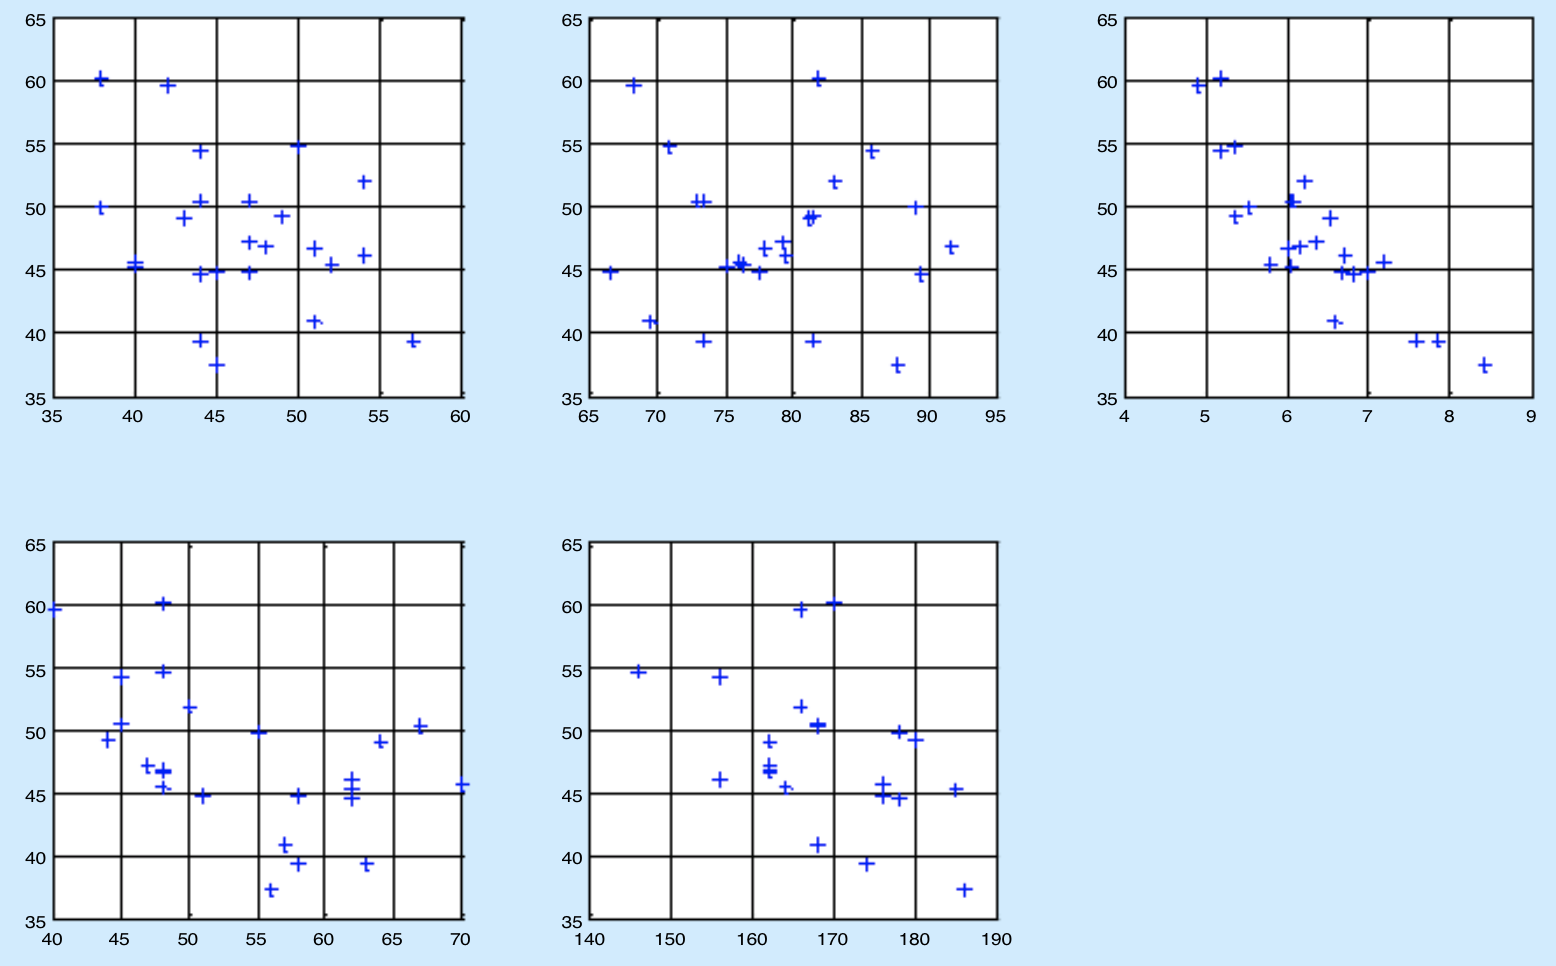
\includegraphics[width=0.8\textwidth]{pic1.png}
\end{figure}

从左到右,从上到下的顺序分别为$x1-x5$的散点图结果。从图中可以看出,除了$x3$自变量呈现比较明显的负相关趋势以外,对于其他的各个自变量都难以直接观测出其对于因变量的影响。根据这个结果,可以假设自变量$x3$(1500m跑后心速)最直接的与锻炼耗氧能力相关,下面通过对各个自变量的单参数回归进行检验。

单参数回归结果:

\begin{table}[H]
\centering
\begin{tabular}{|l|l|l|l|l|l|l|l|}
\hline
对象 &$\beta_0$&$\beta_1$&$\beta$置信区间&$R^2$&F&p&$s^2$\\ \hline
x1 & 64.3812 & -0.3599 & -0.8309,0.1111  & 0.1025 & 2.5115  & 0.1273 & 31.2484 \\ \hline
x2 & 52.7432 & -0.0644 & -0.4334,0.3046  & 0.0059 & 0.1310  & 0.7309 & 34.6097 \\ \hline
x3 & 83.4438 & -5.6682 & -7.1252,-4.2112 & 0.7474 & 65.0959 & 0.0000 & 8.7943  \\ \hline
x4 & 67.1094 & -0.3599 & -0.6262,-0.0936 & 0.2631 & 7.8560  & 0.0104 & 25.6547 \\ \hline
x5 & 94.0024 & -0.2739 & -0.5095,-0.0384 & 0.2091 & 5.869   & 0.0247 & 27.5352 \\ \hline
\end{tabular}
\end{table}

由单参数回归的结果可以证明$x3$(1500m跑后心速)可以最好地反映出y(锻炼耗氧能力)的情况。由$\beta_1$置信区间可以看出,$x1,x2$包含0在内,说明y可能与该参数无关,所以不选择,并且两者的p值已经明显地大于$\alpha=0.05$,因此不考虑$x1,x2$。比较$x3,x4,x5$后发现,$x3$的$R^2$决定系数明显的大于$x4,x5$的决定系数,决定系数反映在因变量的总变化中自变量引起的那部分的比例,$x3$决定系数大说明其对因变量起的决定作用较大。并且$x3$的p和$s^2$值也比较小,所以最终确定$x3$可以最好的反映出y的情况。

用Ploytool检验含$x3$高次(2次)项的情况,参量如下表:

\begin{table}[H]
\centering
\begin{tabular}{|l|l|l|l|l|l|l|l|}
\hline
&$\beta_0$&$\beta_1$&$\beta_2$\\ \hline
回归系数估计值 & 122.7242 & -17.9072 & 0.9356\\ \hline
置信区间下限 & 67.1878 & -35.0387  & -0.3695\\ \hline
置信区间上限 & 178.2605 & -0.7757 & 2.2408\\ \hline

\end{tabular}
\end{table}
\begin{figure}[H]
    \centering
    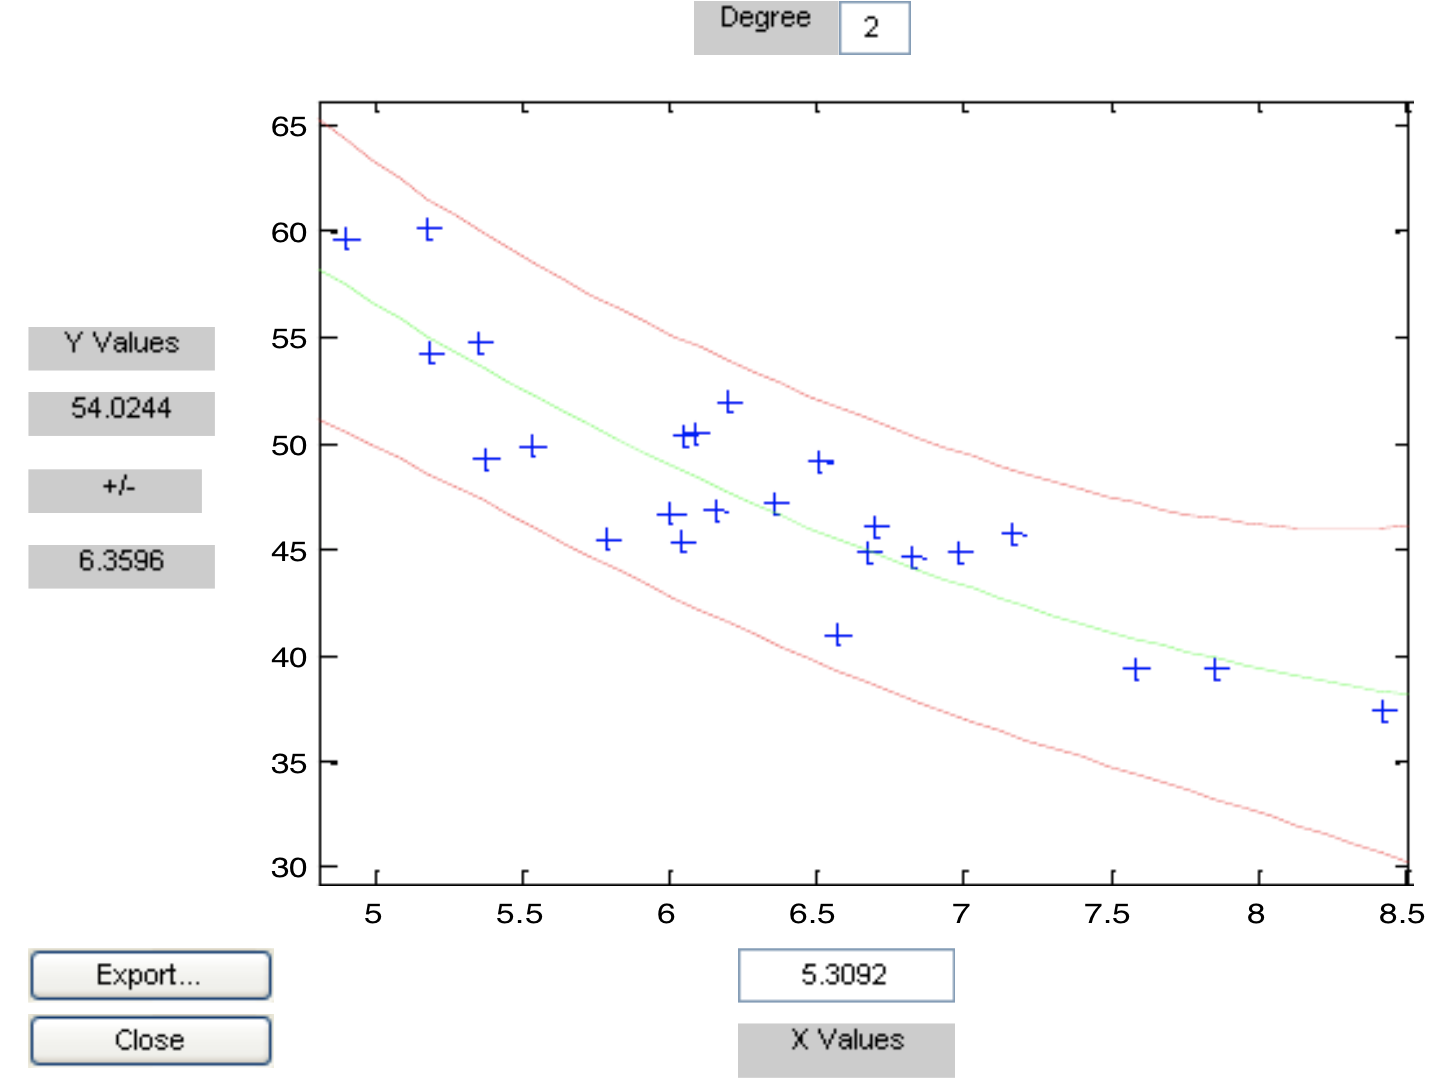
\includegraphics[width=0.5\textwidth]{pic2.png}
\end{figure}

可以同以前仅含一次项的结果进行比较,发现各个参量的置信区间都很宽,且$\beta_2$的置信区间含有0,可以认为二次项的引入是不重要的。

因此采用单参数模型描述y最为准确:

$$y=\beta_0+\beta_3x3, \beta_0=83.4438,\beta_3=-5.6682$$

双参数回归:

用stepwise作逐步回归,主要回归结果如下图:

\begin{figure}[H]
    \centering
    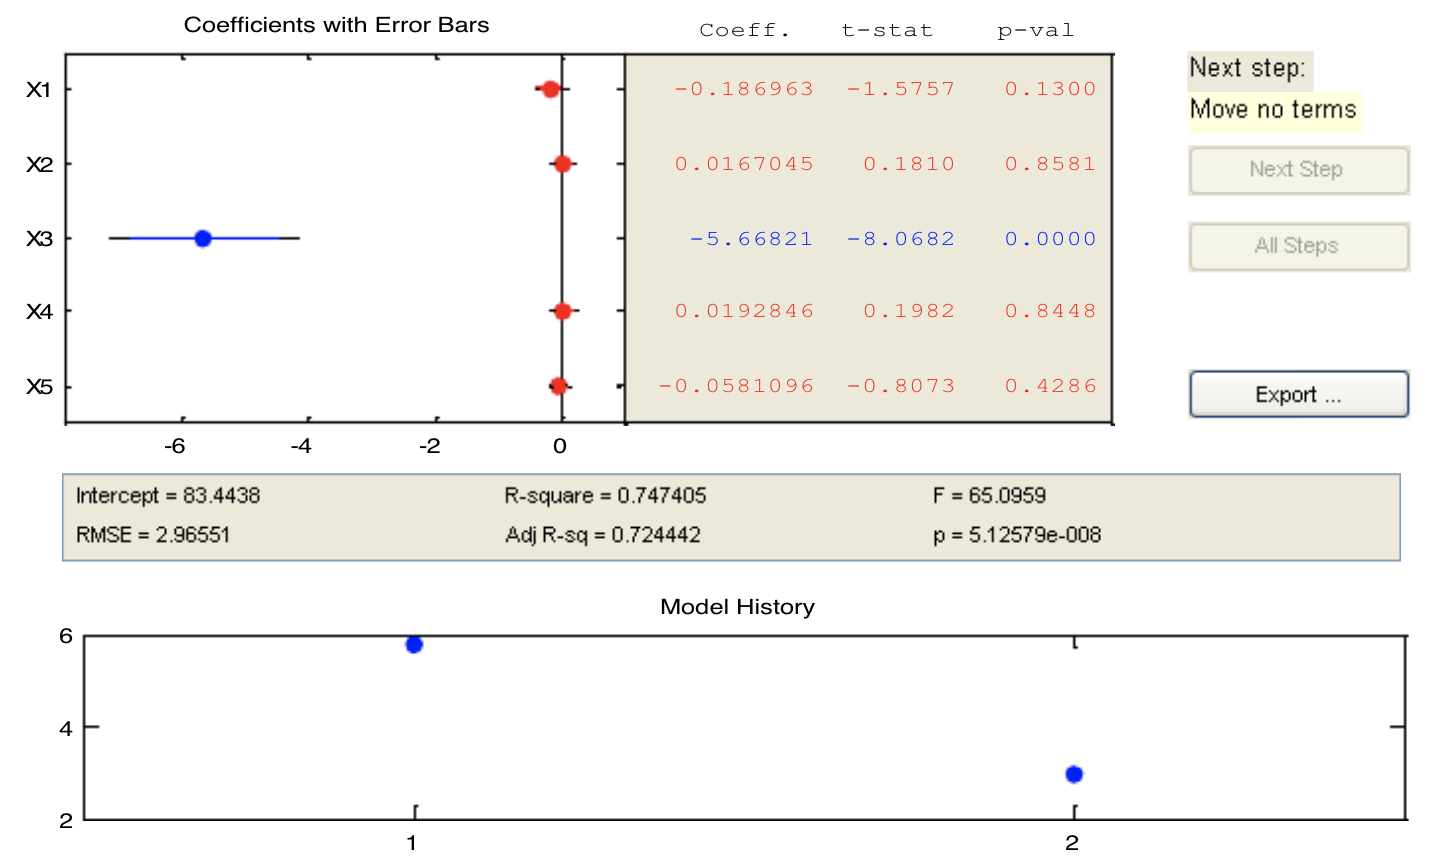
\includegraphics[width=0.5\textwidth]{pic3.png}
    \title{x3 only}
\end{figure}

\begin{figure}[H]
    \centering
    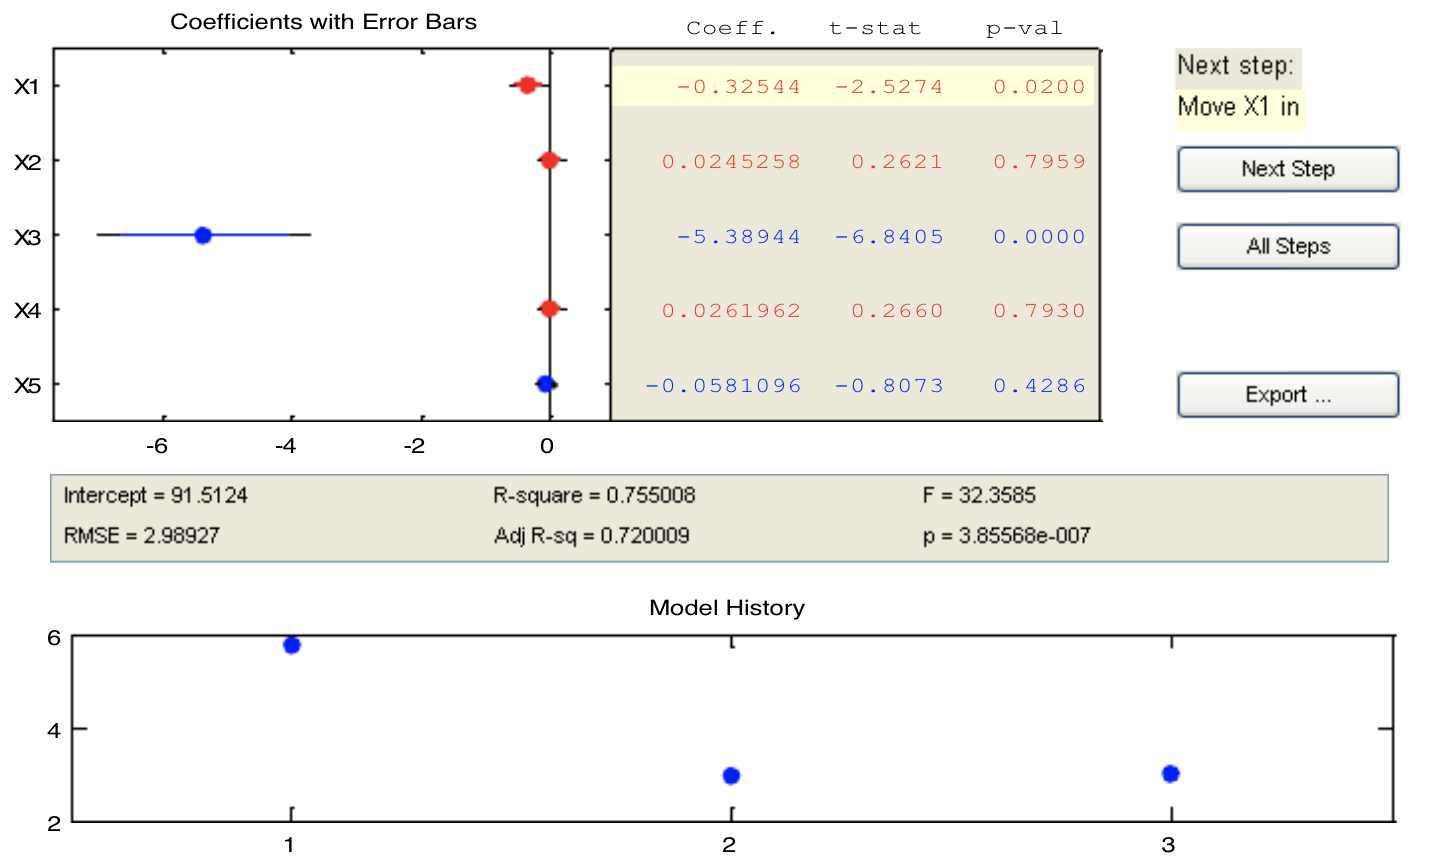
\includegraphics[width=0.5\textwidth]{pic4.png}
    \title{x3 \& x5}
\end{figure}

\begin{figure}[H]
    \centering
    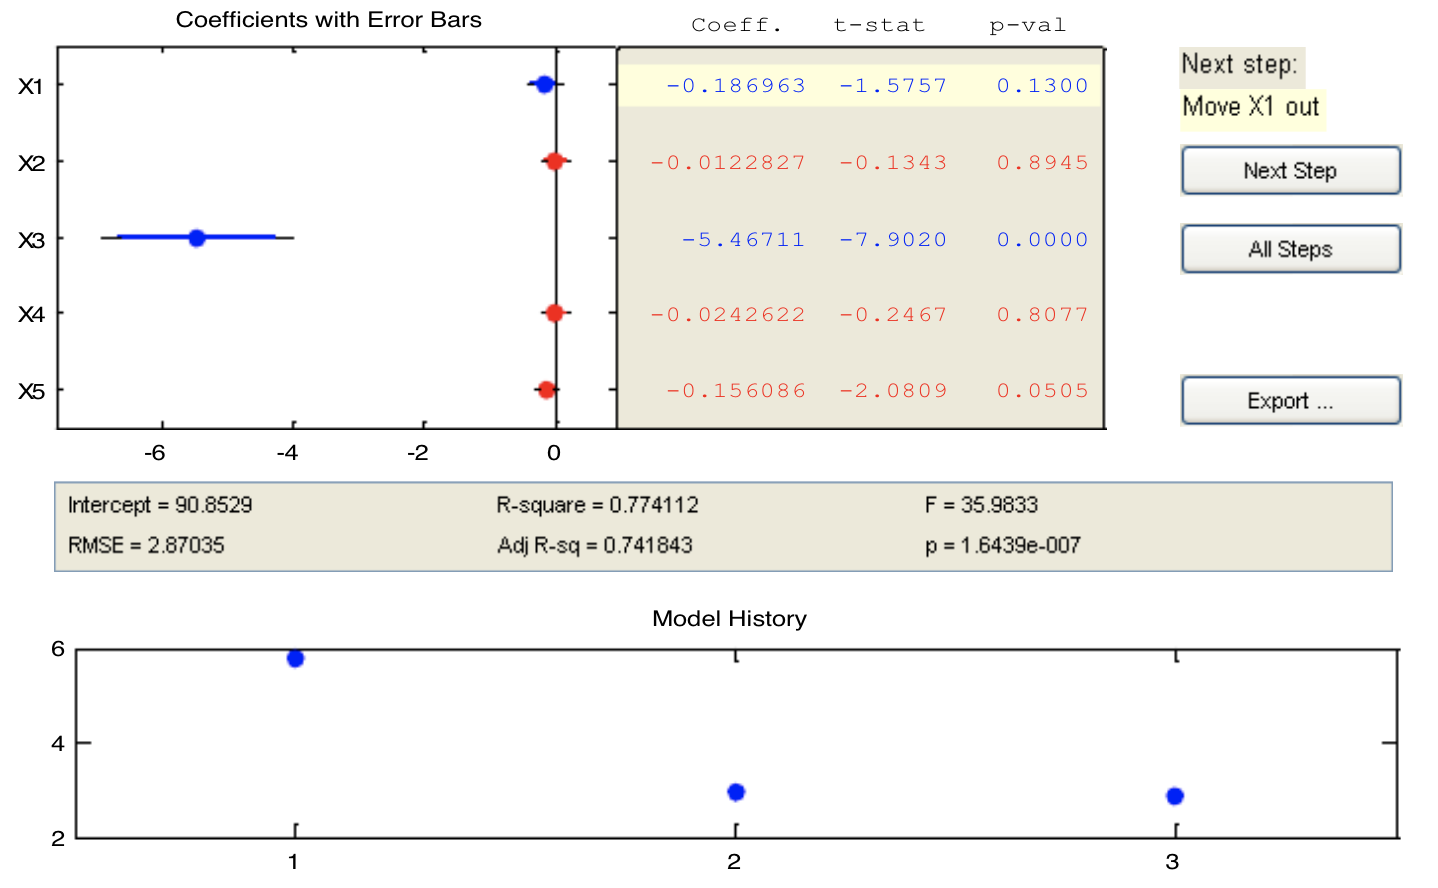
\includegraphics[width=0.5\textwidth]{pic5.png}
    \title{x3 \& x1}
\end{figure}

根据题目要求,最终得到取双参量时的最佳结果是$x3,x1$,即1500m跑后心速和年龄,此时RMSE参量最小。但是实际的追捕回归过程在此时并没有结束,最终的最优结果是只取$x3$参量,这说明取$x1,x3$和取$x3$相比没有很大优势。

通过rstool命令检验二元情况下的交互项和高次项情况,下图是linear情况下固定单参数进行预测的结果:

\begin{figure}[H]
    \centering
    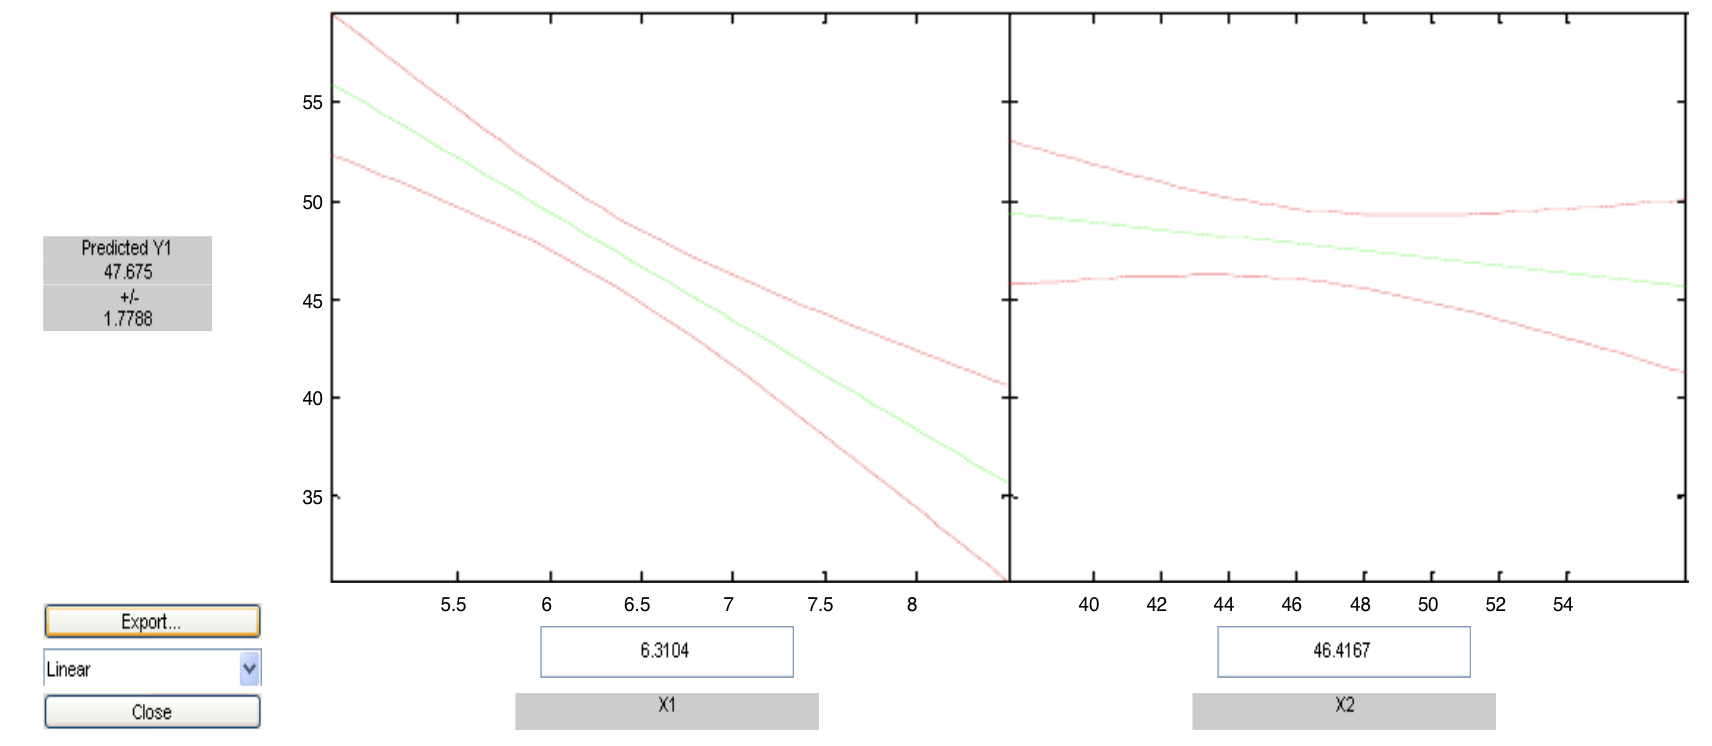
\includegraphics[width=0.8\textwidth]{pic6.png}
\end{figure}

\begin{table}[H]
\centering
\begin{tabular}{|l|l|l|l|l|l|l|l|}
\hline
项对应的系数 &常数项&X3&X1&$X3^2$&$X1^2$&X3*X1&RMSE\\ \hline
Linear & 90.8529& -5.4671 & -0.187  & &  &  & 2.8704 \\ \hline
Purequadratic & 142.8835 & -14.7911 & -1.1718  & 0.7111 & 0.0109  & & 2.9028 \\ \hline
Interaction & 120.1929 & -10.1096 & -0.8364 &   &  & 0.1025 & 2.9033  \\ \hline
Quadratic & 144.4666 & -16.4515 & -1.0199 & 0.0405 & 0.6818  & 0.0062 & 2.9786 \\ \hline
\end{tabular}
\end{table}

可以看到高次项和相关项的系数都非常小,说明其对于y的影响不大。根据RMSE的结果进行比较,仍选择linear回归方式,即只用二元变量的一次项。

$$y=\beta_0+\beta_1x_1+\beta_3x_3,\quad \beta_0=90.8529,\beta_1=-0.1870,\beta_3=-5.4671$$

全参数回归:

根据以上的分析可以验证模型建立时的猜想,本题中5个自变量和y的关系都不是很直接的,除$x3$以外的其他变量影响很小,因此在最终完整模型中,不考虑高次项和交互项的影响,以简化模型和节省筛选时间。

采用stepwise命令,仅对五个自变量的一次项进行回归分析,结果如下:
\begin{figure}[H]
    \centering
    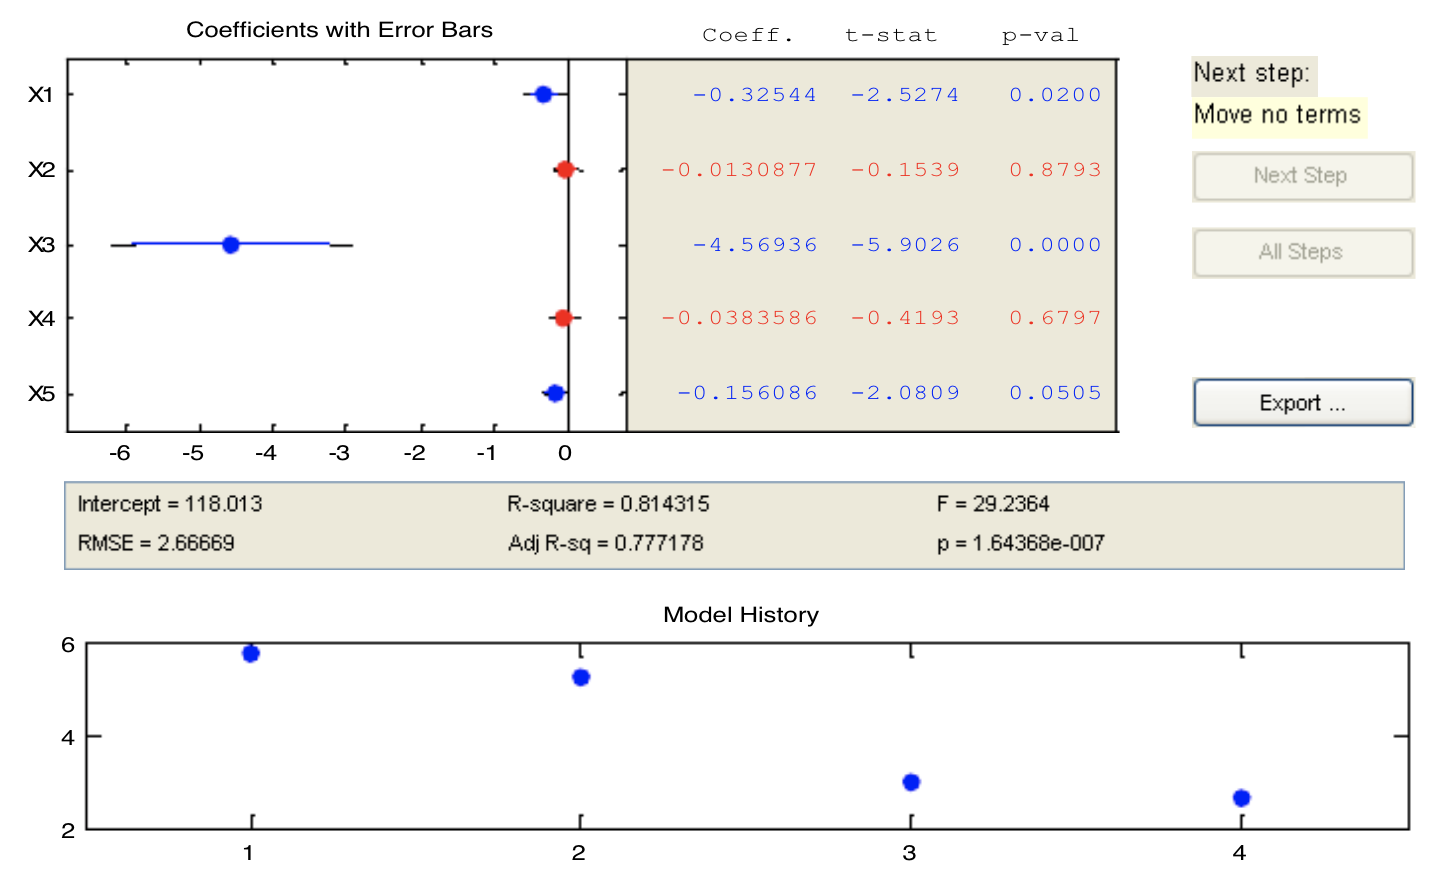
\includegraphics[width=0.8\textwidth]{pic7.png}
\end{figure}

参数结果为:

\begin{table}[H]
\centering
\begin{tabular}{|l|l|l|l|l|l|l|l|}
\hline
 &$\beta$&置信区间&Coeff&se&t-stat&p-val\\ \hline
x1 & -0.3254 & -0.594,-0.0568 & -0.3254  & 0.1288 & -2.5274  &0.02\\ \hline
x2 & 0 & 0,0 & -0.0131 & 0.0851 & -0.1539  & 0.8793 \\ \hline
x3 & -4.5694 & -6.1842,-2.9546 & -4.5694 & 0.7741 & -5.9026 & 0  \\ \hline
x4 & 0 & 0,0 & -0.0384 & 0.0915 & -0.4193  & 0.6797 \\ \hline
x5 & -0.1561 & -0.3126,0.0004 & -0.1561 & 0.075 & -2.0809  & 0.0505 \\ \hline
\end{tabular}
\end{table}

$$R^2=0.814315,F=29.2364,RMSE=2.66669,P=1.64368e-7$$

最终取以下三个参数得到最佳回归结果:$x3,x1,x5$,即1500m跑后心速、年龄和跑步后心速。但是仍需要进行一般回归分析确定常数项并观察残差,结果如下:


\begin{figure}[H]
    \centering
    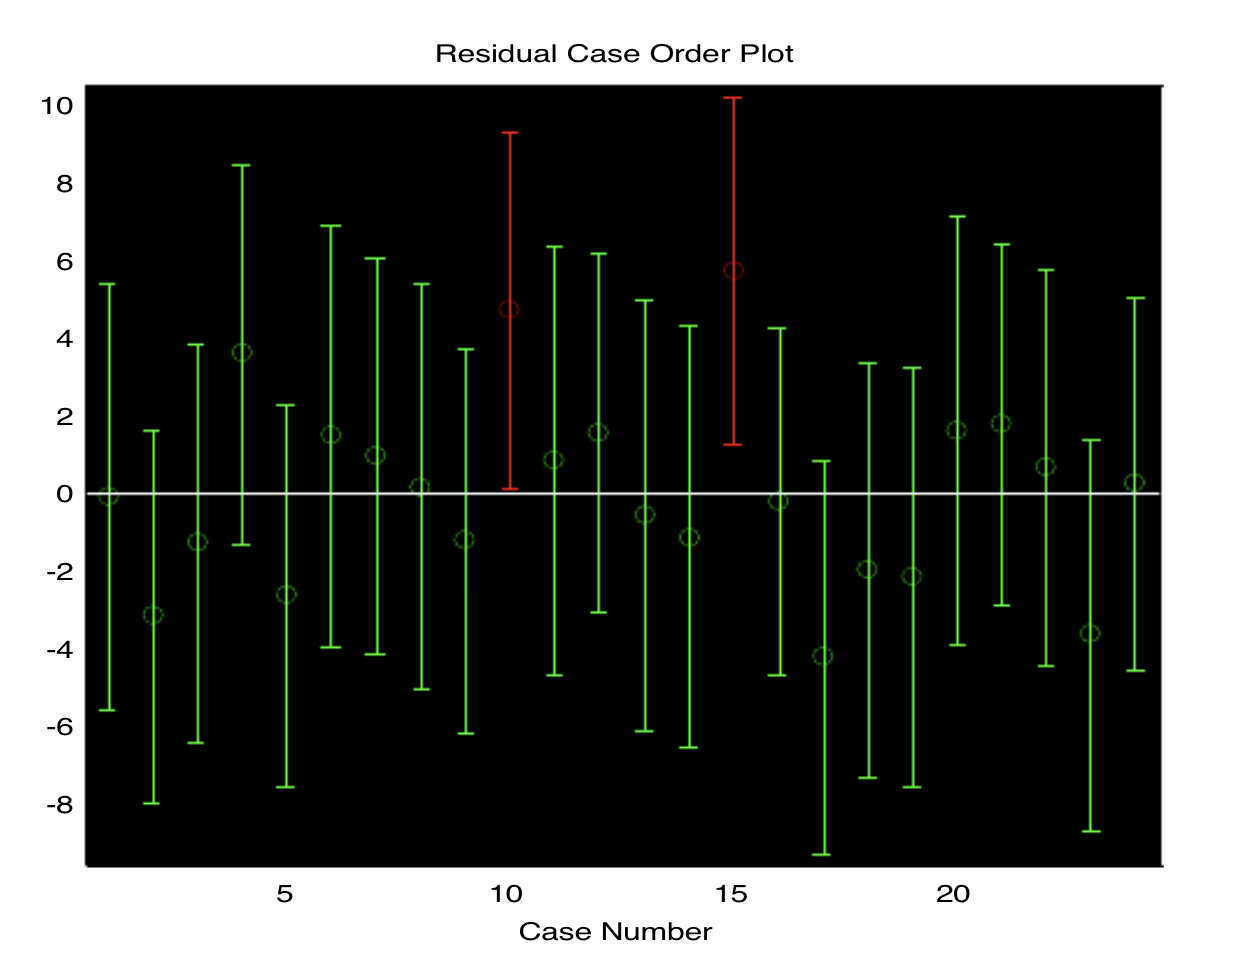
\includegraphics[width=0.8\textwidth]{pic8.png}
\end{figure}

可以看到10和15号数据异常进行剔除操作继续观察。

\begin{figure}[H]
    \centering
    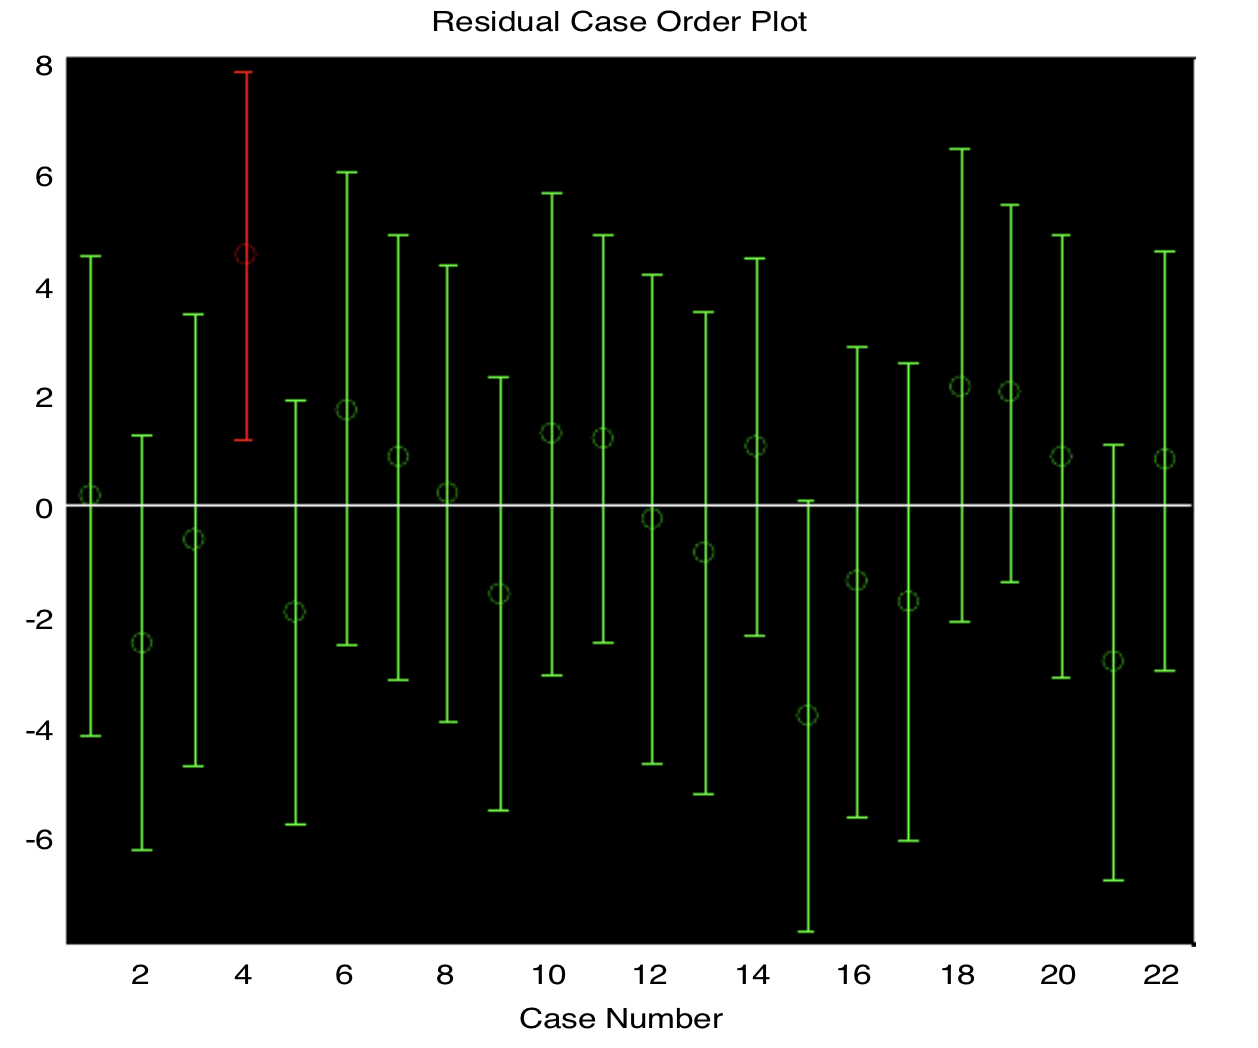
\includegraphics[width=0.8\textwidth]{pic9.png}
\end{figure}

可以看到4号数据异常,进行剔除操作。

最终经过4次剔除操作,去掉了5个数据点(4、10、15、17、23),得到了没有异常点的模型:

\begin{figure}[H]
    \centering
    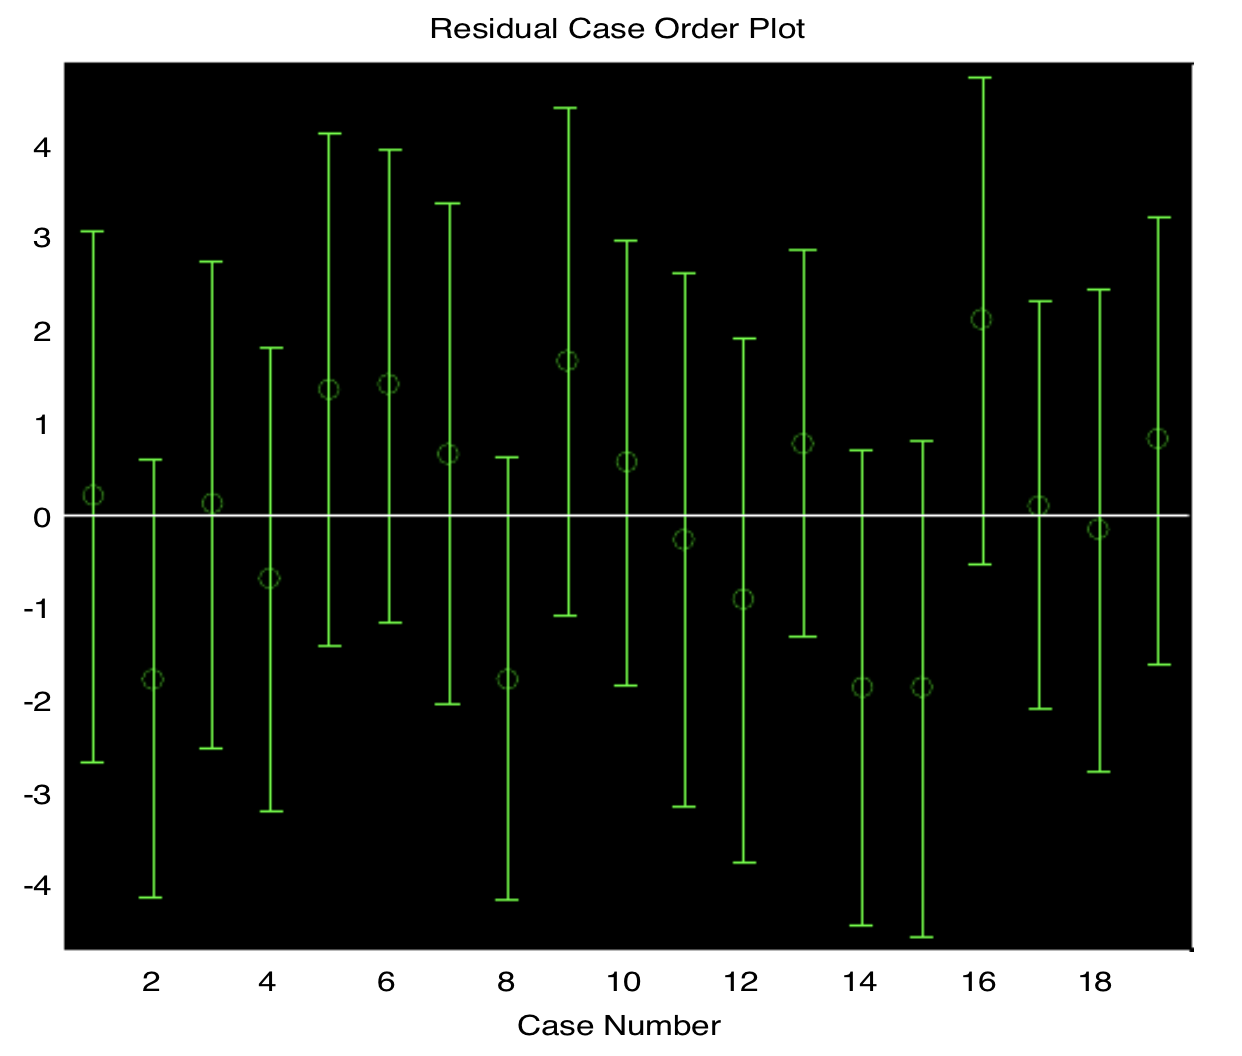
\includegraphics[width=0.8\textwidth]{pic10.png}
\end{figure}

最终得到的结果整体上优越于剔除异常点之前的结果(不再粘贴结果)。但是事实上,由于 数据点经过剔除不断的结果,模型最终的形式和实际统计到的24组数据的整体情况偏离越
来越大,也就是说:剔除异常点虽然能够一应程度上降低其对于整体情况的干扰作用,而剔 除的过程也放大了其他原本正常数据点的异常性,所以异常点可能会不断产生,但是剔除的 数量增加即采样数据的减少也会削弱模型反省整体性能的能力。是一对矛盾,在数据点较少 的时候尤其明显。比较科学的做法是:只进行1次或少次剔除,保证整体性,又去掉了最主 要的异常点。


这里的最终结果采用剔除最初两个异常点(10, 15号)后的结果,在此也附上完整数 据(剔除之前)的结果,作为第3问的答案:

完整数据(第三题结果):
\begin{table}[H]
\centering
\begin{tabular}{|l|l|l|}
\hline
回归参数 & 取值       & 置信区间             \\ \hline
$\beta_0$     & 118.0135 & 88.1010,147.9260 \\ \hline
$\beta_1$     & -0.3254  & -0.5940,-0.0568  \\ \hline
$\beta_3$     & -4.5694  & -6.1842,-2.9546  \\ \hline
$\beta_5$     & -0.1561  & -0.3126,0.0004   \\ \hline
\end{tabular}
\end{table}

$$R^2=0.8143,F=29.2364,p=0.0000,s^2=7.1112$$

$$y=\beta_0+\beta_1x_1+\beta_3x_3+\beta_5x_5,\quad \beta_0=118.0135,\beta_1=-0.3254,\beta_3=-4.5694,\beta_5=-0.1561$$


一次剔除(最终结果):
\begin{table}[H]
\centering
\begin{tabular}{|l|l|l|}
\hline
回归参数 & 取值       & 置信区间             \\ \hline
$\beta_0$     & 119.4955 & 94.6827,144.3084 \\ \hline
$\beta_1$     & -0.3623  & -0.5991,-0.1255  \\ \hline
$\beta_3$     & -4.0411  & -5.3617,-2.7205  \\ \hline
$\beta_5$     & -0.1774  & -0.3030,0.0518   \\ \hline
\end{tabular}
\end{table}

$$R^2=0.8625,F=37.6269,p=0.0000,s^2=4.400$$

$$y=\beta_0+\beta_1x_1+\beta_3x_3+\beta_5x_5,\quad \beta_0=119.4955,\beta_1=-0.3623,\beta_3=-4.0411,\beta_5=-0.1774$$


通过上篇幅的讨论可以得到,1500m跑后心速、年龄和跑后心速这三个参数最能够反映锻炼耗氧量这个重要的身体状态指标。心跳速度越快,耗氧量越大,速度越慢,即时间越长,耗氧量越小。


\section{CH13-T9 洗衣粉制造}
\subsection{模型设计与建立}

与第一个问题类似,我们使用线性回归法进行拟合,模型基本形式如下:

$$y=\beta_0+\beta_1x_1+\cdots+\beta_mx_m+\sum_{i\leq j,k\leq m}\beta_{jk}x_jx_k+\xi$$

\subsection{计算结果与分析}

基本代码实现:

\begin{lstlisting}
y = [...];
x1 = [1 1 1 1 1 2 2 2 2 2 3 3 3 3 3];
x2 = [6 7 8 9 10 6 7 8 9 10 6 7 8 9 10];

figure(1),plot(x1,y,'*');
figure(2),plot(x2,y,'*');

X1 = [x1',x2'];
stepwise(X1, y)
n=15;
X2=[ones(n,1),x1',x2'];
[b,bint,r,rint,s]=regress(y',X2);
rcoplot(r,rint)

\end{lstlisting}

下图为搅拌程度与泡沫高度关系图(左)和洗衣粉用量与泡沫高度关系图(右)。

\begin{figure}[H]
    \centering
    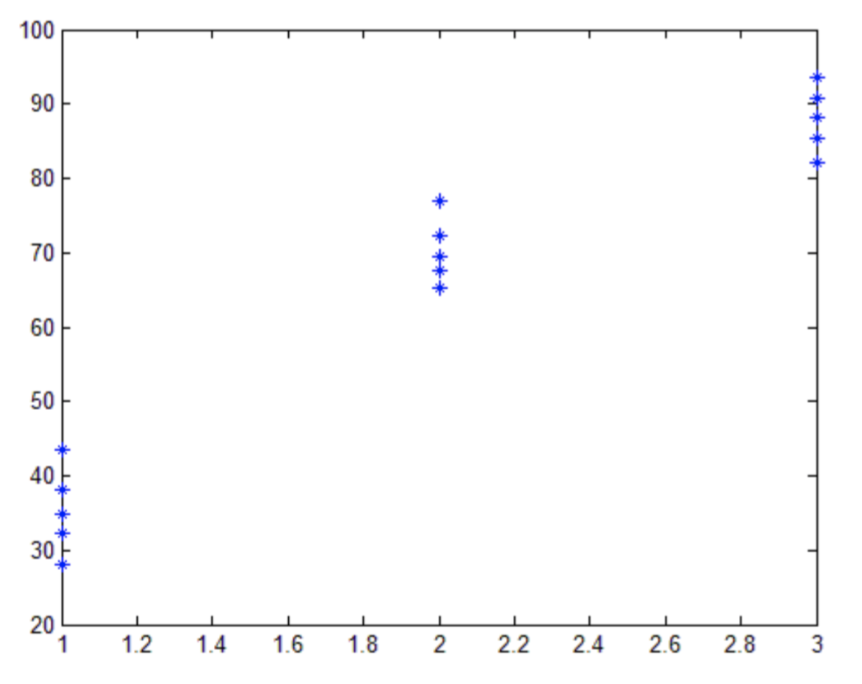
\includegraphics[width=0.4\textwidth]{pic11.png}
    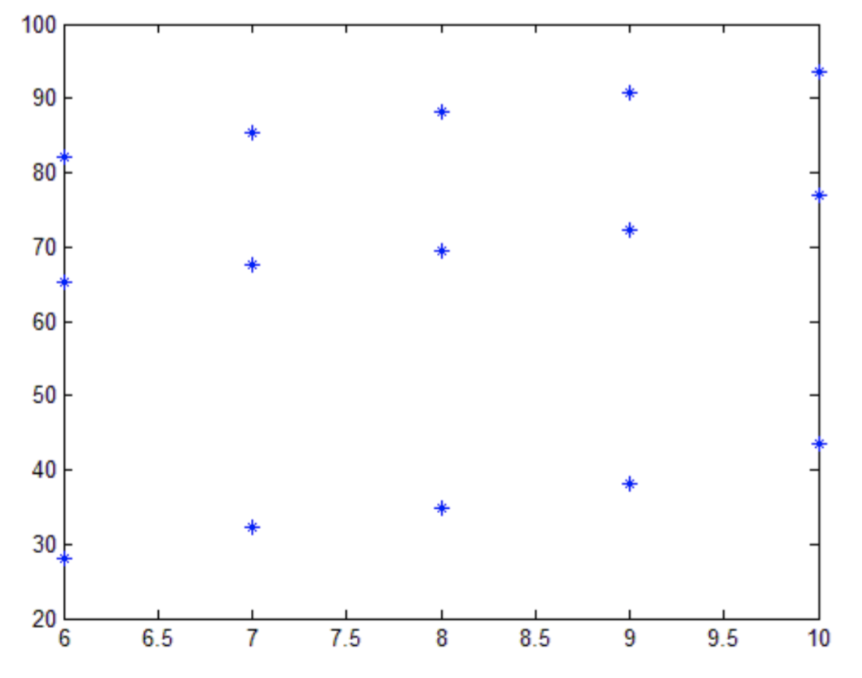
\includegraphics[width=0.4\textwidth]{pic12.png}
\end{figure}


\begin{figure}[H]
    \centering
    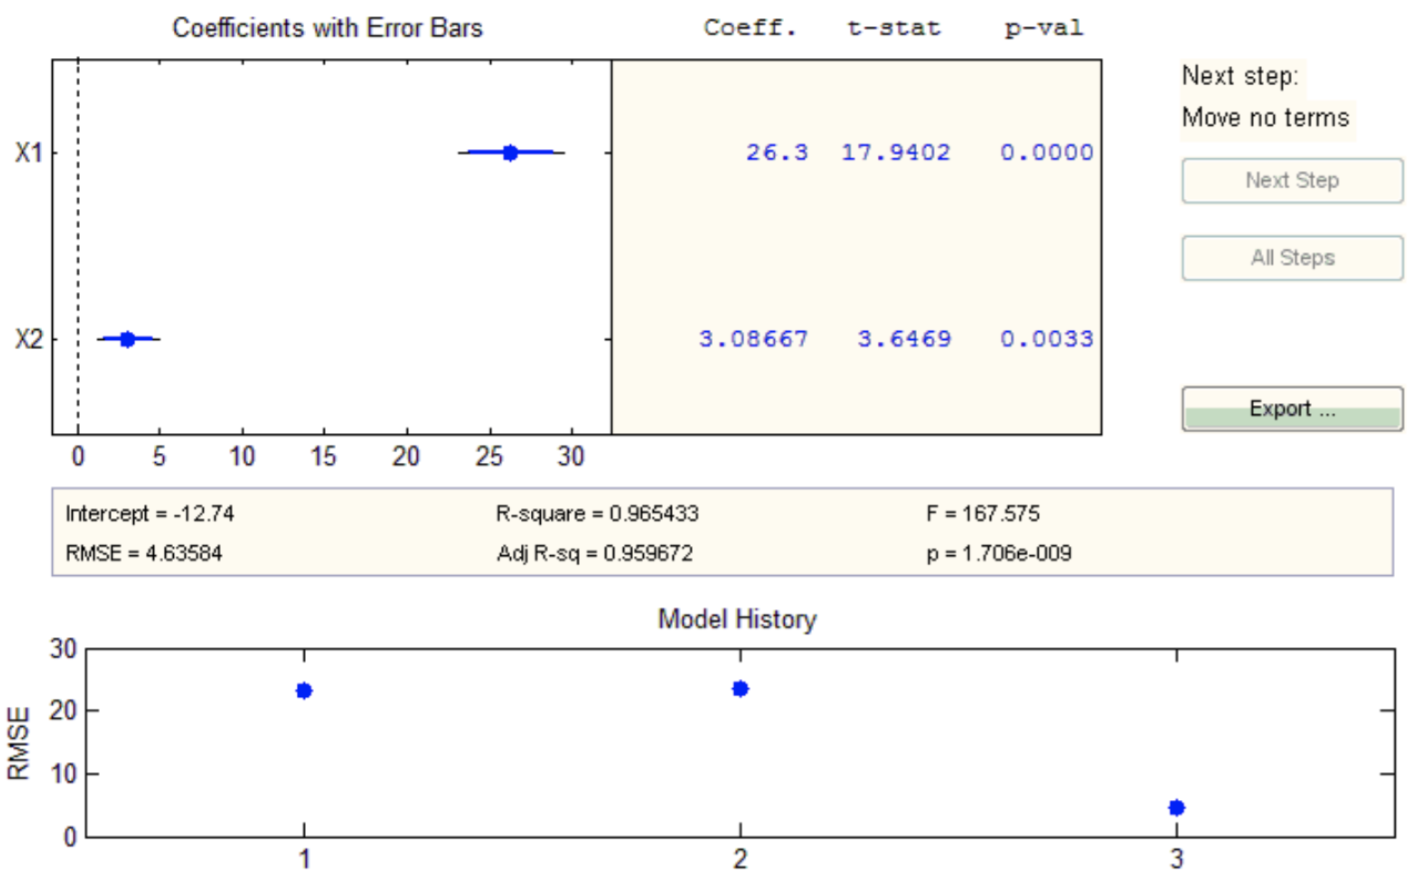
\includegraphics[width=0.8\textwidth]{pic13.png}
\end{figure}

根据提示得到当含有$x1,x2$两项是RMSE最小,因此模型建立为:

$$y=\beta_0+\beta_1x_1+\beta_2x_2,\quad \beta_0=-12.74,\beta_1=26.3,\beta_2=3.08667$$

进行残差分析可以得到:


\begin{figure}[H]
    \centering
    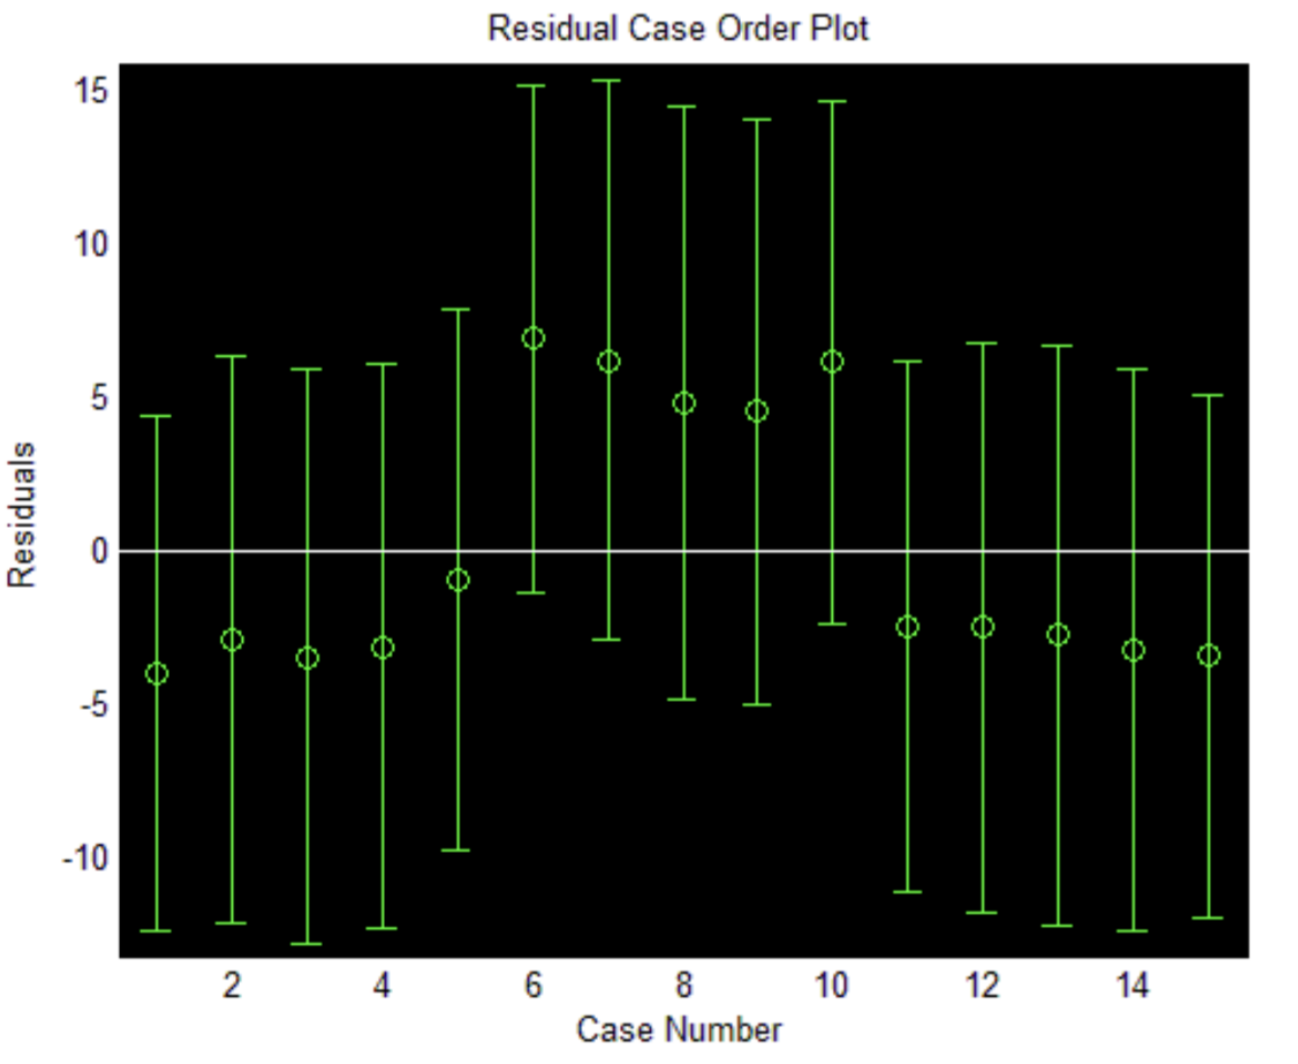
\includegraphics[width=0.8\textwidth]{pic14.png}
\end{figure}

可以看到中等搅拌程度的残差明显与其他不同。

下面将搅拌程度用0-1表示,进行泡沫高度关系分析。

\begin{lstlisting}
y = [...];
x0 = [0 0 0 0 0 0 0 0 0 0 1 1 1 1 1];
x1 = [0 0 0 0 0 1 1 1 1 1 0 0 0 0 0];
x2 = [6 7 8 9 10 6 7 8 9 10 6 7 8 9 10];

figure(1),plot(x0,y,'*');
figure(2),plot(x1,y,'*');
figure(3),plot(x2,y,'*');

X1 = [x0',x1',x2'];
stepwise(X1, y)
n=15;
X2=[ones(n,1),x0',x1',x2'];
[b,bint,r,rint,s]=regress(y',X2);
rcoplot(r,rint)

\end{lstlisting}

我们不妨设$x0,x1$共同表示搅拌程度,当$(x0,x1)=(0,0)$时,表示搅拌程度为1,当$(x0,x1)=(0,1)$时,表示搅拌程度为2,当$(x0,x1)=(1,0)$时,表示搅拌程度为3。

得到的分析结果如下:

y与$x1,x2,x3$的关系散点图为:

\begin{figure}[H]
    \centering
    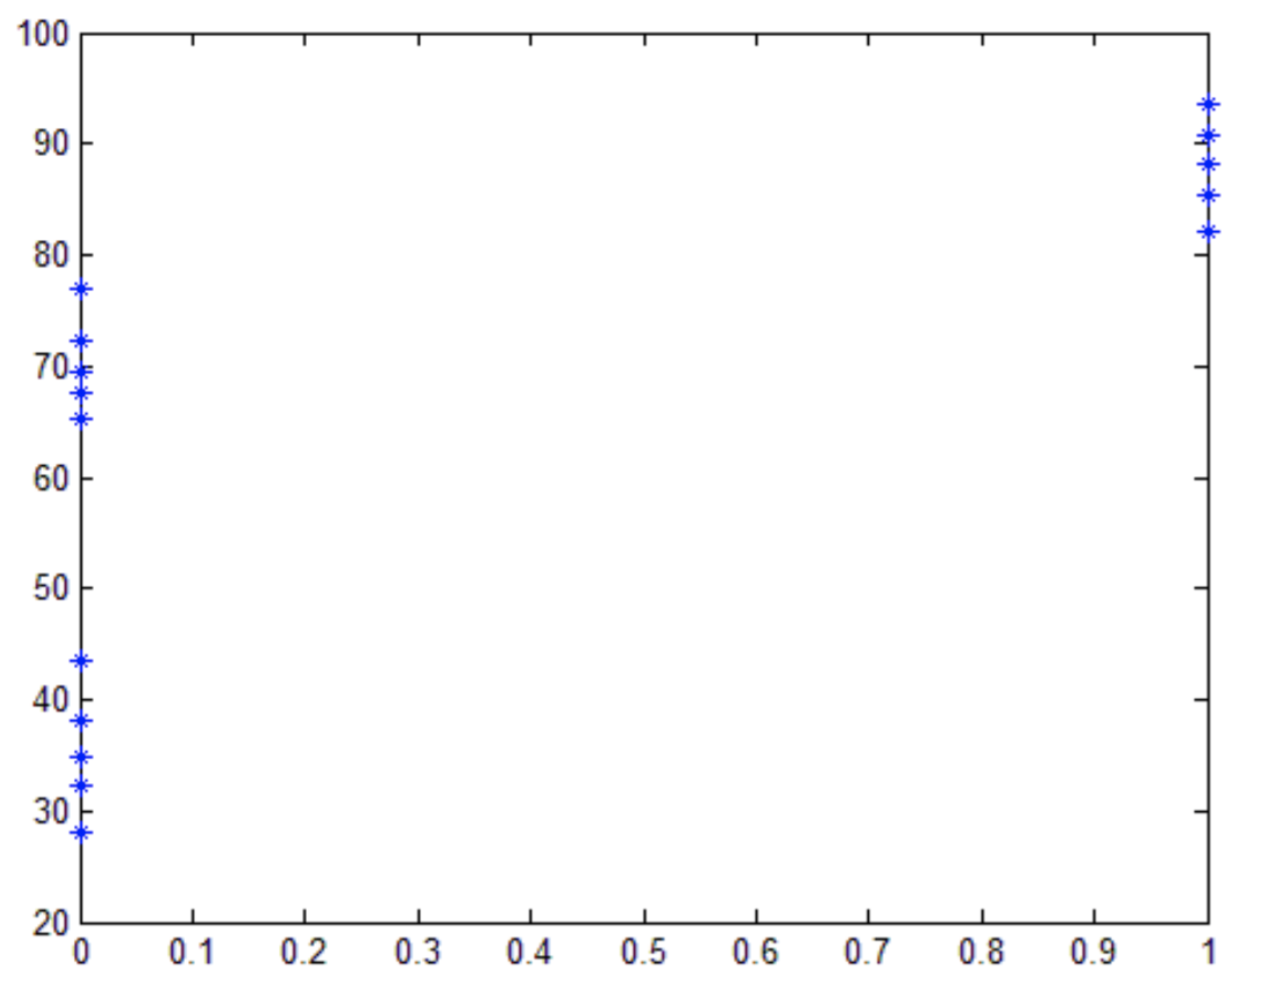
\includegraphics[width=0.4\textwidth]{pic15.png}
    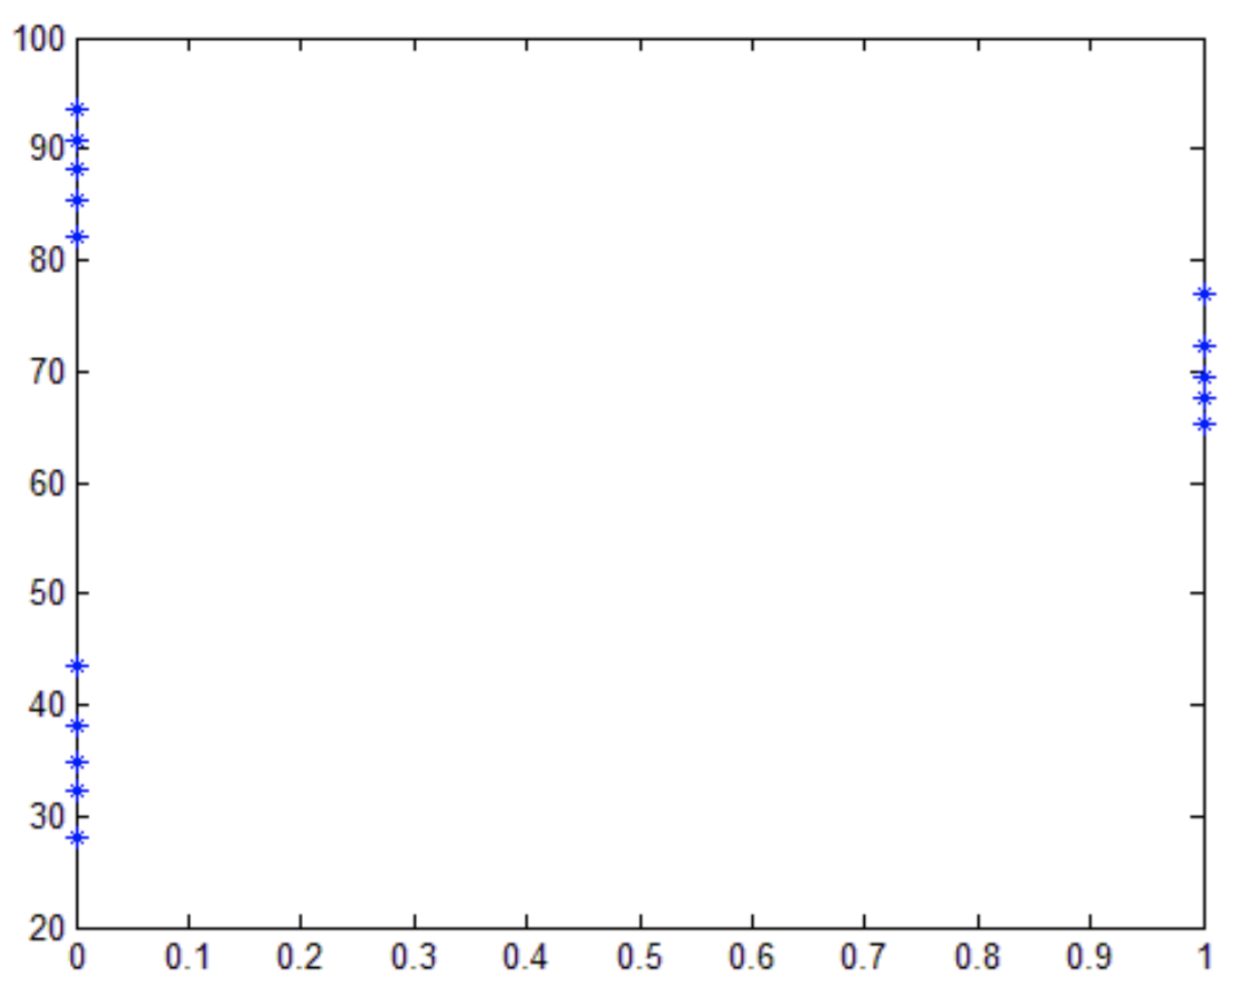
\includegraphics[width=0.4\textwidth]{pic16.png}
    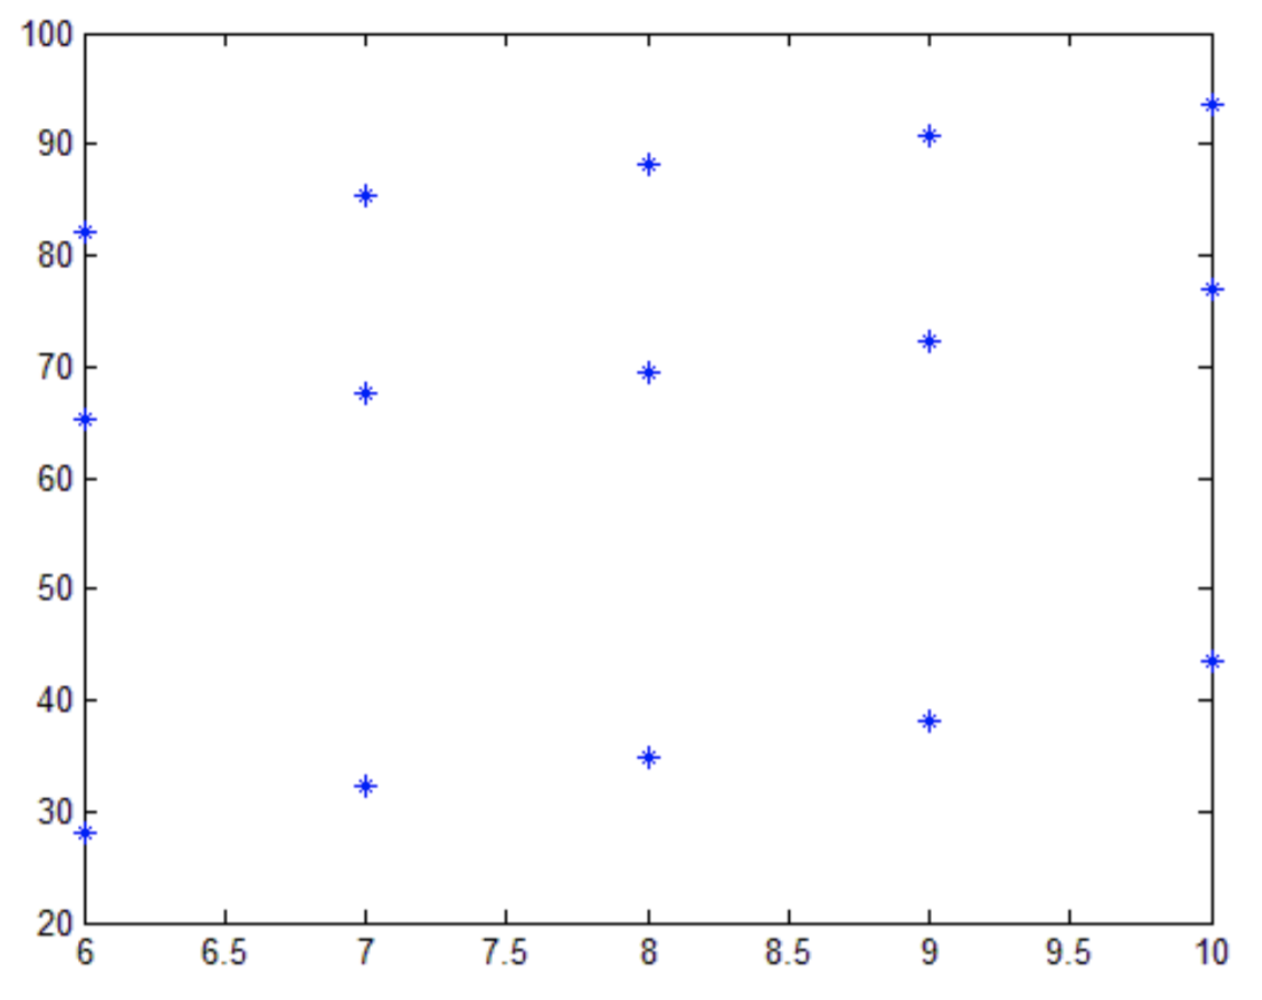
\includegraphics[width=0.4\textwidth]{pic17.png}
\end{figure}

\begin{figure}[H]
    \centering
    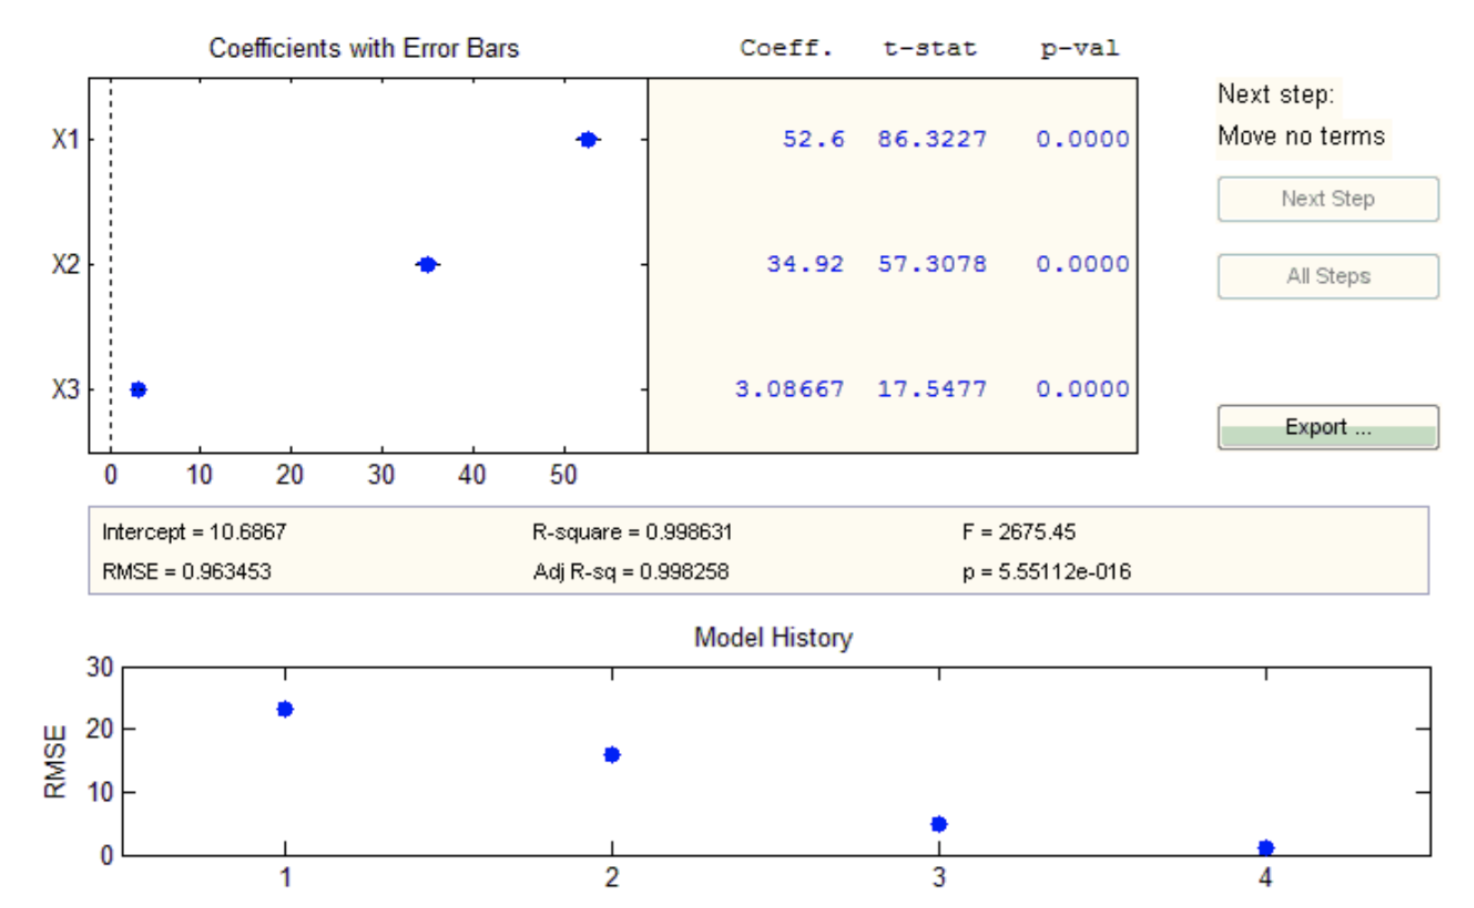
\includegraphics[width=0.8\textwidth]{pic18.png}
\end{figure}

可以看出当RMSE最小时含有$x0,x1,x2$项,,此时模型建立为:

$$y=\beta +\beta_0x_0+\beta_1x_1+\beta_2x_2,\quad\beta=10.6867,\beta_0=52.6,\beta_1=34.92,\beta_2=3.08667$$

残差分析结果如下图:

\begin{figure}[H]
    \centering
    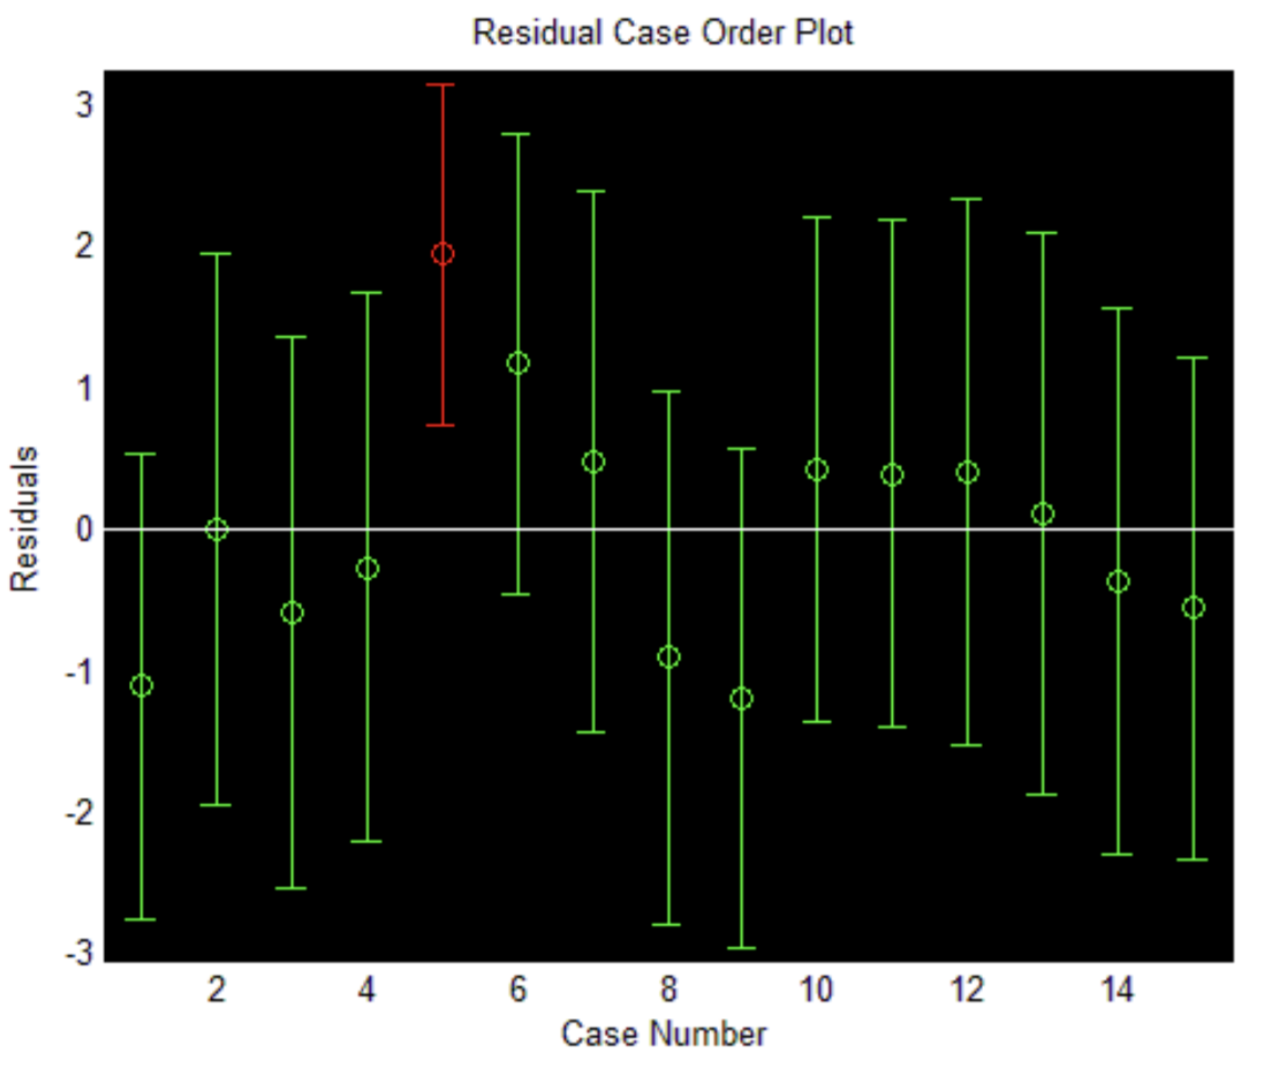
\includegraphics[width=0.8\textwidth]{pic19.png}
\end{figure}

发现第五组数据应该剔除,剔除后在此进行残差分析得到下图:

\begin{figure}[H]
    \centering
    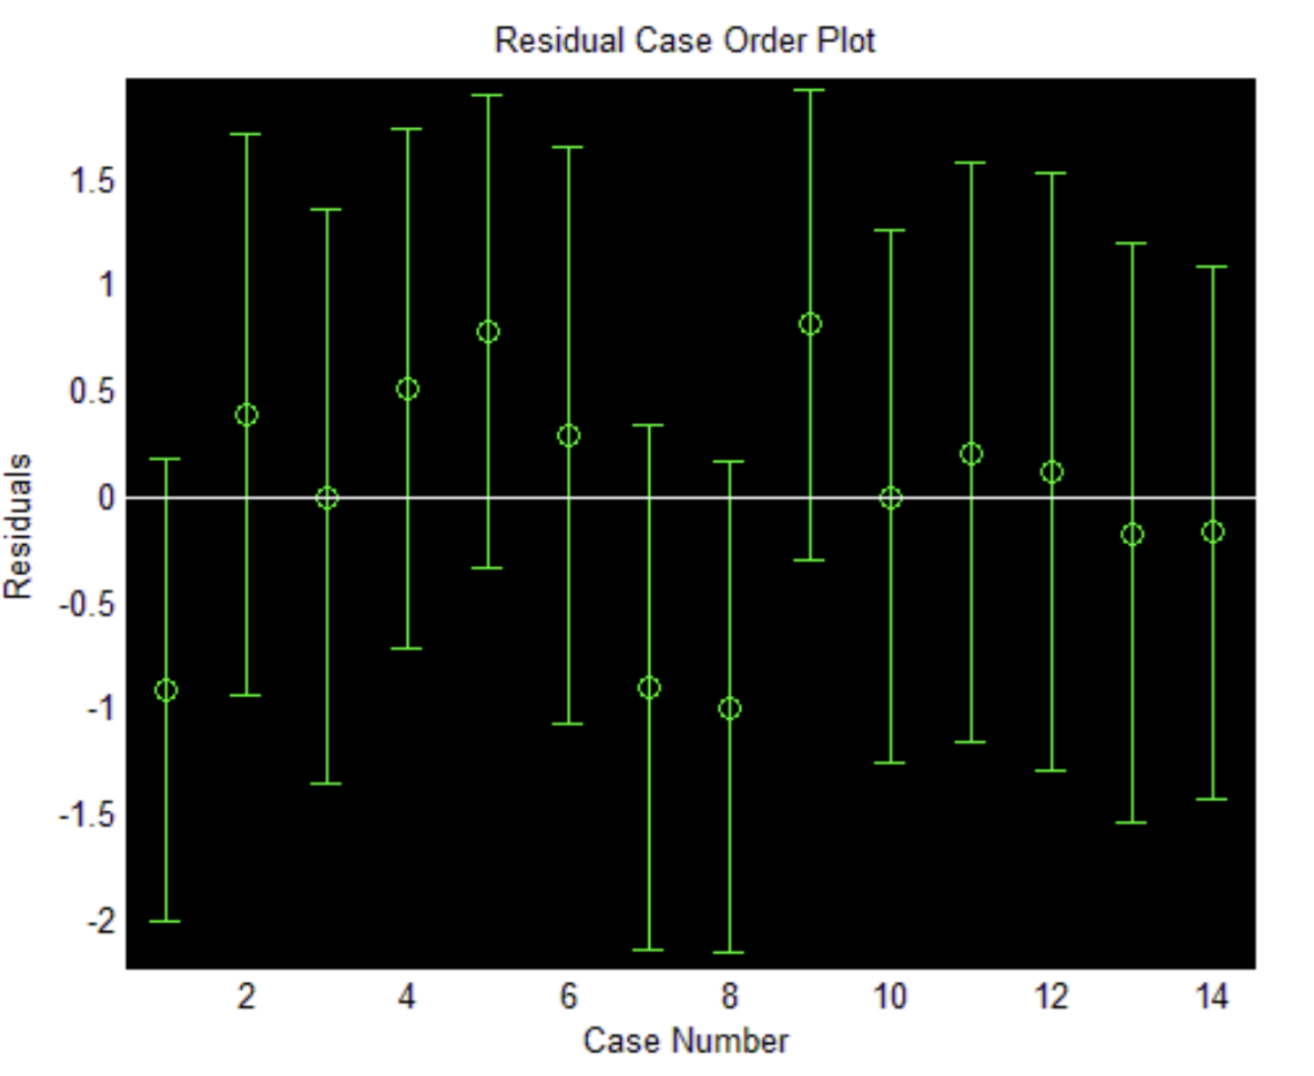
\includegraphics[width=0.8\textwidth]{pic20.png}
\end{figure}

而这时的回归结果为:

\begin{figure}[H]
    \centering
    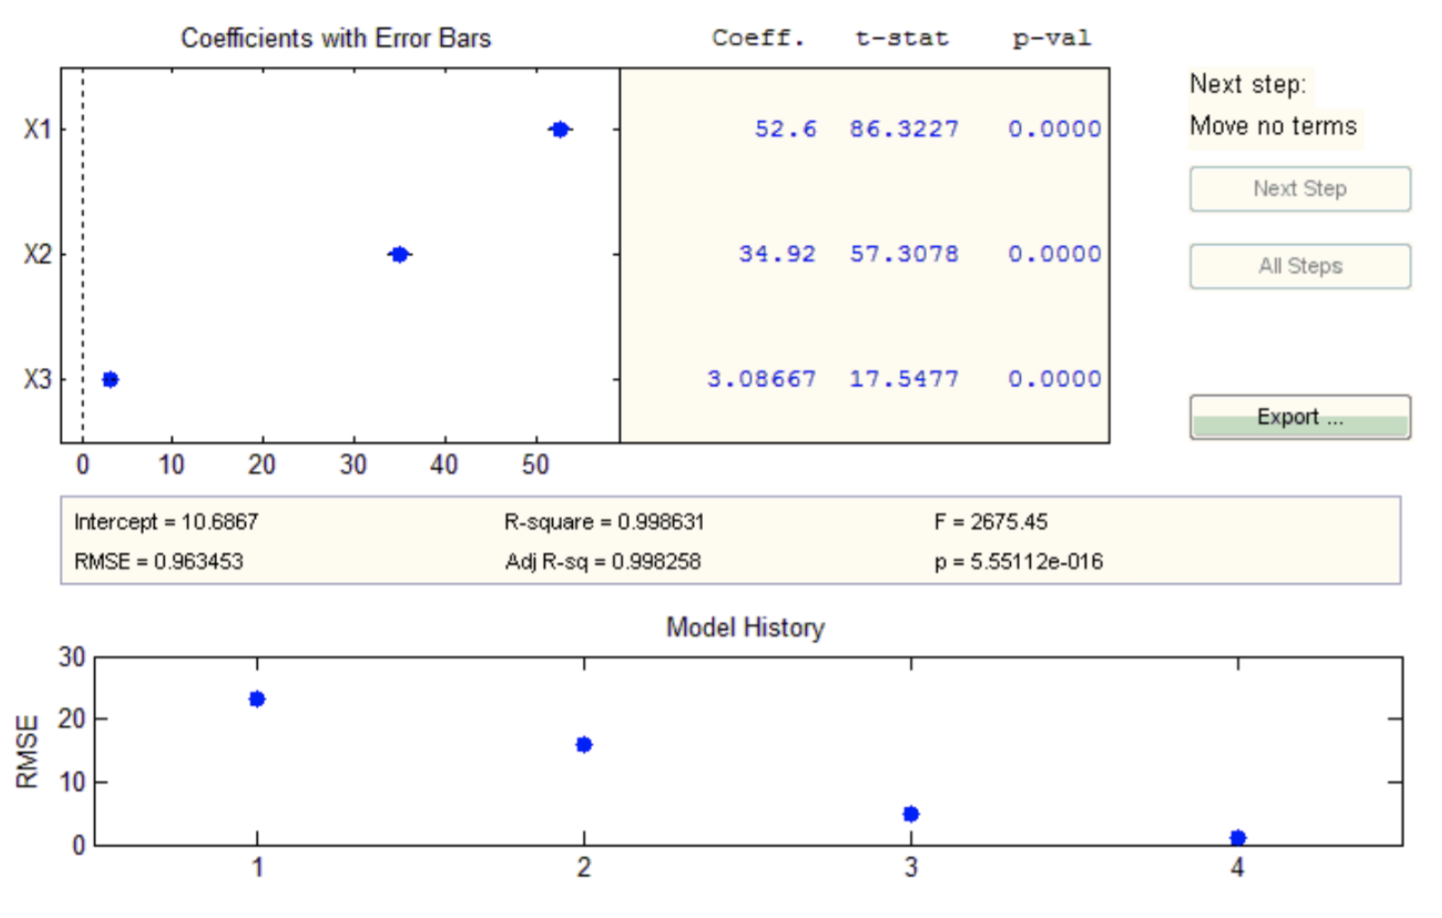
\includegraphics[width=0.8\textwidth]{pic21.png}
\end{figure}

此时模型修改为:

$$y=\beta +\beta_0x_0+\beta_1x_1+\beta_2x_2,\quad\beta=11.66,\beta_0=53.184,\beta_1=35.504,\beta_2=2.892$$


下面将交互项考虑进来分析,结果如下:

\begin{figure}[H]
    \centering
    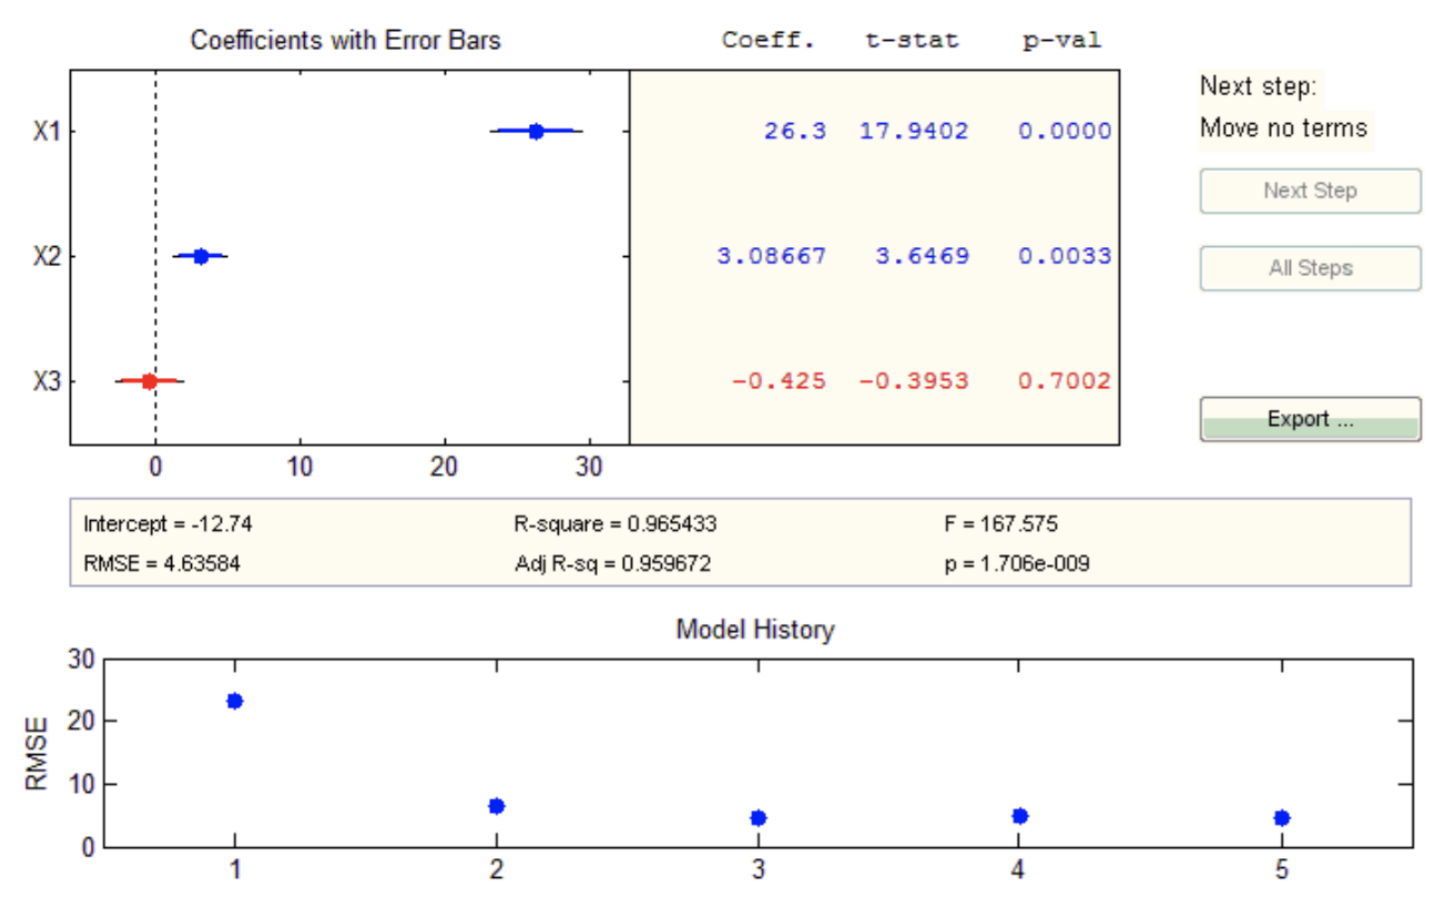
\includegraphics[width=0.8\textwidth]{pic22.png}
\end{figure}

上图为搅拌程度为普通变量的运行结果。

\begin{figure}[H]
    \centering
    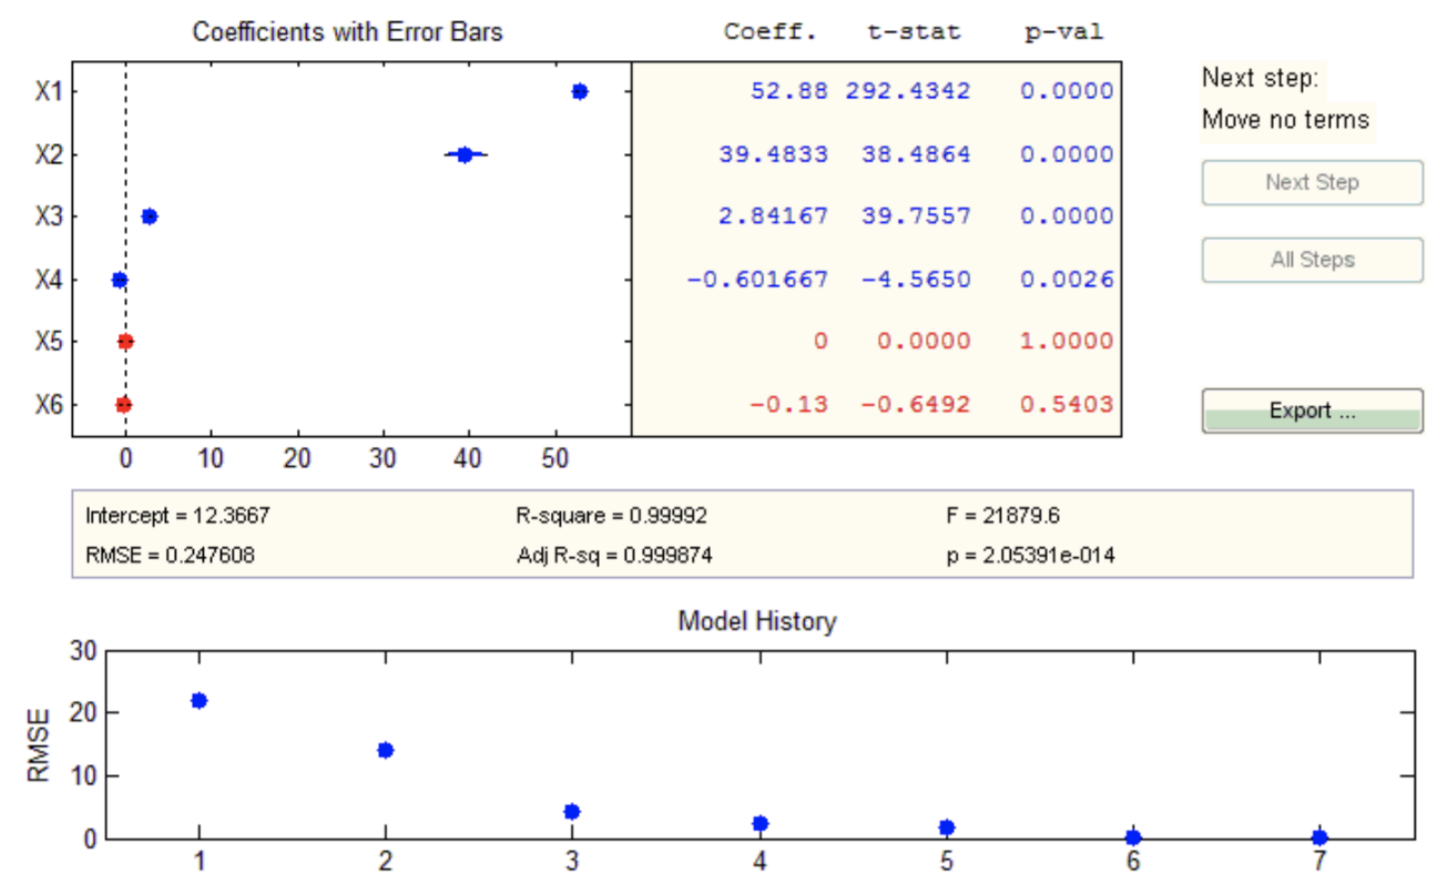
\includegraphics[width=0.8\textwidth]{pic23.png}
\end{figure}

上图为搅拌程度为0-1表示的运行结果。

可以看到,当搅拌程度表示为普通变量时,交互项没有对模型进行任何的改进,模型仍然为:

$$y=\beta_0+\beta_1x_1+\beta_2x_2,\quad \beta_0=-12.74,\beta_1=26.3,\beta_2=3.08667$$

当搅拌程度用0-1表示时,交互项会改进模型,改进后的模型为:

$$y=\beta +\beta_0x_0+\beta_1x_1+\beta_2x_2+\beta_{12}x_1x_2$$
$$\beta=12.3667,\beta_0=52.88,\beta_1=39.4833,\beta_2=2.84167,\beta_{12}=-0.601667$$


\section{CH13-T13 高压锅销量}
\subsection{线性拟合}

由表中给出的数据,假设y和t满足线性关系,因此建立线性模型,设模型为:

$$y = a + kx$$

利用最小二乘法确定$a,k$的具体指,并根据$a,k$的值拟合高压锅的销售情况,与原数据进行比较。

MATLAB代码如下:

\begin{lstlisting}
y = [43.65 109.86 187.21 312.67 496.58 707.65 960.25 1238.75 1560.00 1824.29 2199.00 2438.89 2737.71];
t = 0:12;
p = polyfit(t,y,1);
yy = polyval(p,t,1);
plot(t,y,'*',t,yy)

\end{lstlisting}

通过计算可以得到:

$$a=-279.4818,k=236.5355$$

原数据与拟合的曲线为:

\begin{figure}[H]
    \centering
    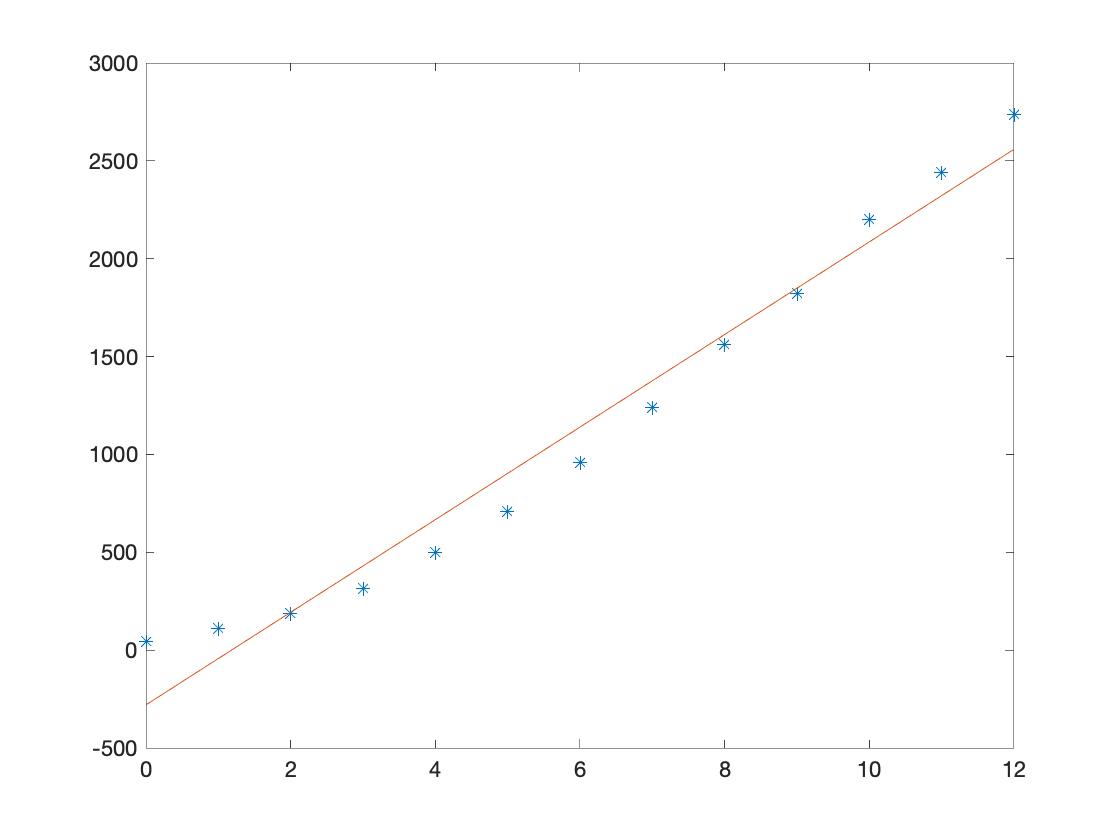
\includegraphics[width=0.8\textwidth]{pic24.png}
\end{figure}

下面进行误差分析:

线性模型的误差分析我们采用如下的预测标准误差:

$$s=\sqrt{\frac{(yy-y)^2}{13}}=157.2915$$

可以看到线性模型虽然简单,但是误差很大。并且当t趋向于无穷时,y趋向于无穷,这是不符合常理的。根据生活常识可以指导高压锅的销售量是有限的,也就是高腰过的销售量最终是一个有限的数,不能达到无穷大。

所以用线性模型不能够完全反映高压锅的销售情况,必须去寻找一个更好的模型。

\subsection{非线性回归}

由于高压锅在进入市场初期没有多少人家了解或清楚高压锅,致使人们对高压锅的购买数量不大,所以此时高压锅销售数量的增长率小;随着时间的推移,人们开始认识到使 用高压锅的好处,高压锅的销售量增长率也逐渐提高;之后越来越多的人家都有高压锅了, 而高压锅的经久耐用决定了高压锅销售量的增长率会逐渐减少;到最后该地区基本上所有 人家都有高压锅了,高压锅的销售数量将趋于一个定值,即L,此时销售数量的增长率将 趋于0.

所以,综上所述,高压锅的销售情况满足Logistic模型。

使用Matlab对Logistic模型做非线性回归代码如下:


\begin{lstlisting}
y = [43.65 109.86 187.21 312.67 496.58 707.65 960.25 1238.75 1560.00 1824.29 2199.00 2438.89 2737.71];
t = 0:12;
L = 3000;
y1 = log(L./y-1);
p = polyfit(t,y1,1);
k = -p(1)
a = exp(p(2));
yy = L./(1+a*exp(-k*t));
plot(t,y,'*',t,yy)

\end{lstlisting}

可以得到:

$$s = 0.0002, k=0.4574$$

\begin{figure}[H]
    \centering
    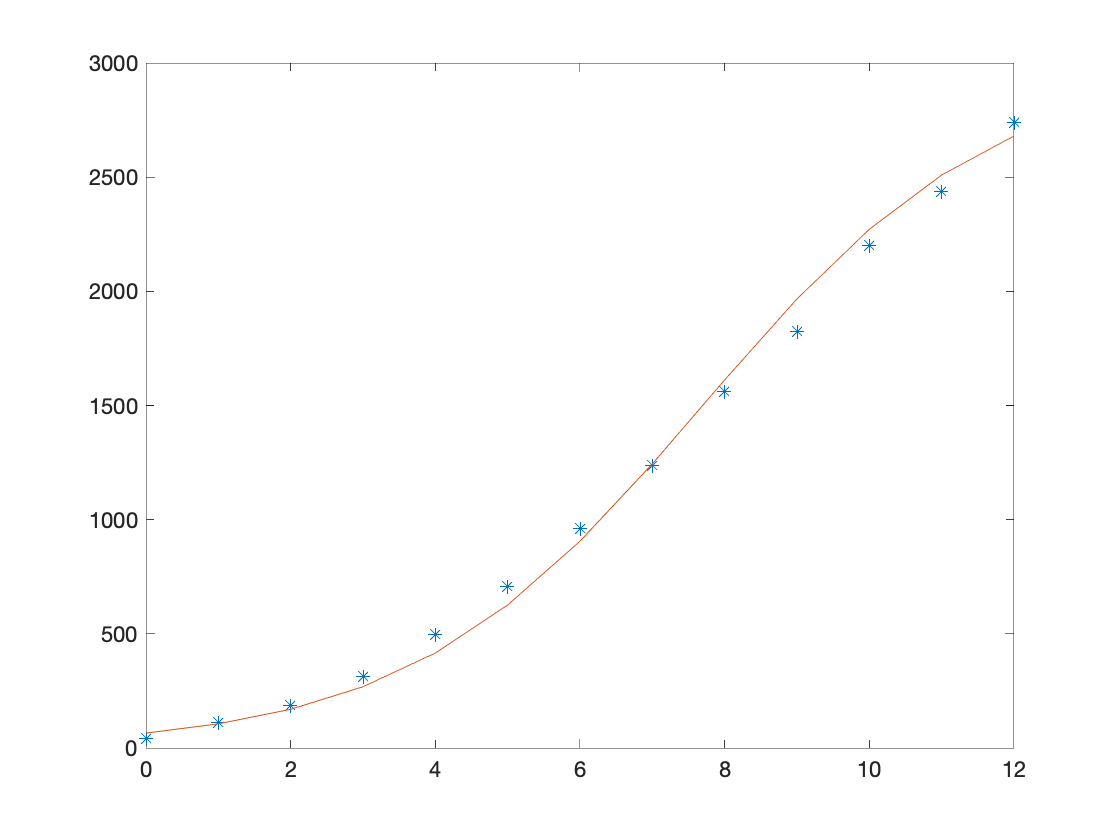
\includegraphics[width=0.8\textwidth]{pic25.png}
\end{figure}

可以看到,在$y=y_m/2$的时候曲线斜率最大,也就是高压锅的销量增长率最大,这与我们建立的模型实际情况比较吻合,而且从图中可以看到,大部分点可以很好的与曲线吻合。

模型检验:

当估计模型参数的时候舍去以后一个数据点,即1993年实际销量数据的时候,我们可以在得到模型参数后计算模型估计值与实际值做模型的检验。

去掉最后一个数据点计算得到的参数为:

$$s = 0.0002, k=0.4574$$

$$y_{(12)}=\frac{3000}{1+30.01e^{-0.4574*12}}=2781.6$$

可以看到模型计算出的销量与实际销量的误差为1.6\%,可以认为模型有较好的符合程度,较为精确。


销量预测:

类似的,我们可以通过模型预测下一年的销量,通过计算可以得到下图,图中绿色为拟合曲线,它两侧的红线为置信区间。

\begin{figure}[H]
    \centering
    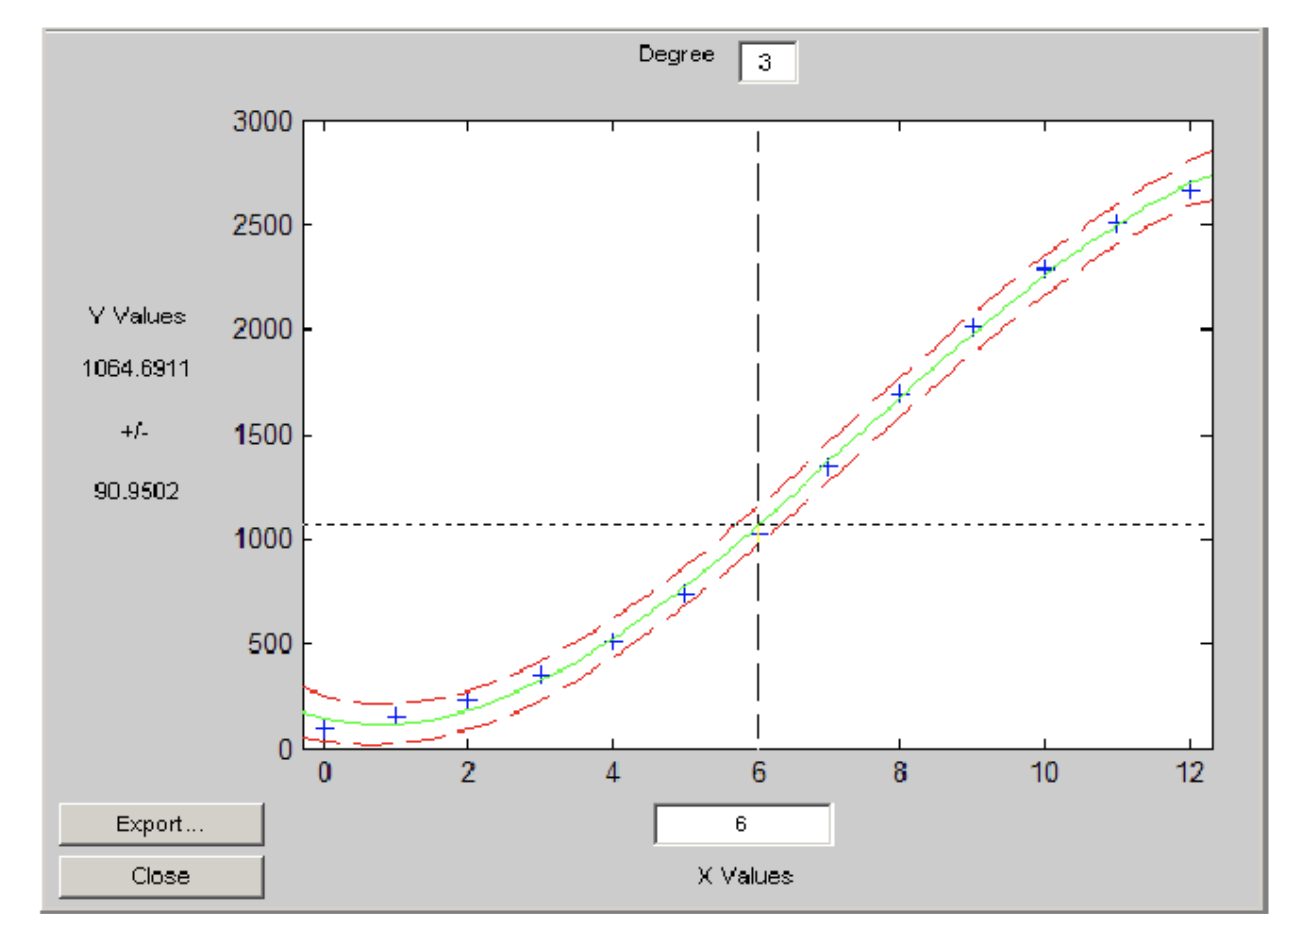
\includegraphics[width=0.8\textwidth]{pic26.png}
\end{figure}

\subsection{拟合Gompertz模型}

MATLAB代码如下:

\begin{lstlisting}
y = [43.65 109.86 187.21 312.67 496.58 707.65 960.25 1238.75 1560.00 1824.29 2199.00 2438.89 2737.71];
t = 0:12;
L = 3000;
y1 = log(log(y/L));
a = polyfit(t,y1,1);
b = -exp(a(2));
k = -a(1);
yy = L*exp(-b*exp(-k*t));
plot(t,y,'*',t,yy);

\end{lstlisting}

得到的拟合曲线为:

\begin{figure}[H]
    \centering
    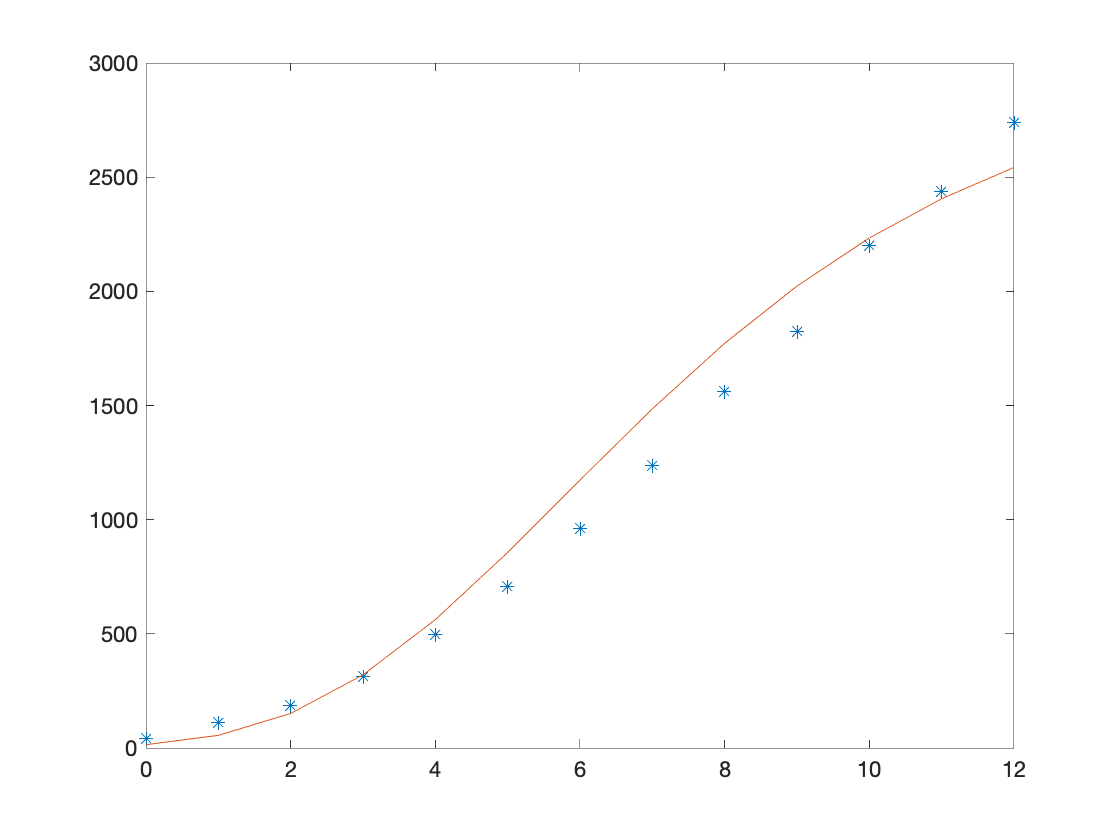
\includegraphics[width=0.8\textwidth]{pic27.png}
\end{figure}

\subsection{总结}
在本题中,我们通过不通的方法对高压锅的销量的增长这一问题建立起来了三个不通的模型,下 
面对这三个模型进行一下比较。

首先是表示高压锅销量的线性增长模型,从图中可以看出在后六年的时间段内,与实际的销量是比较吻合的。但是因为模型与实际情况偏离太大,我们可以注意到随着时间的推移,带来的差距就会越来越大。所以用此模型来 预测高压锅的销量所得出的结果与实际数据可能会存在很大差距。

其次是Logistic组织增长模型,在这个例子中除了中间有几个点不大好 
之外,开始与最后都吻合的很好,尤其是最后的走向与实际销量的趋势吻合的十分完美。 
所以用次模型来预测高压锅的销量所得结果会较为理想。

最后是Gompertz增长模型,在此例中该模型中间段的数据与实际销量 
相差较大,但是从总体的曲线的走势来说,还是与实际相符合的,所以用此模型所作的预 
测还是具有一定的可信度。

通过上面的比较我们发现在此例中,Logistic模型是其中最优的一个。

\section{收获与建议}

通过这次的实验,我学会了使用 MATLAB 求解回归分析问题的一般方法,并对回归分 析的知识有了更深的理解。希望在之后的课堂上老师能够当堂进行相关的技巧演示并给出题 目的分步解答。

本讲的内容实际上和目前很火的机器学习领域关系非常密切,希望老师也能够适当引入 这方面的内容,与时俱进。非常感谢老师和助教这学期的辛苦付出。

\end{document}